\chapter{Data, Trigger and Event Selection}

\section{Data}

Since March 2011 CMS has been taking proton-proton collisions data at $7
\unit{TeV}$ centre of mass energy. A higher centre of mass energy increases the 
production cross-section of certain processes, for example stong production 
SUSY, and also enables the production of more massive particles. It should be 
noted that the important energy is not the centre of mass energy of the proton 
collision, but that of the parton collision which is $\sim 1 \unit{TeV}$ on 
average. \\

The luminosity has increased over time. As the integrated luminosity 
increases more data are available to improve the significance of 
observations and the accuracy of measurements. The luminosity has been increased
by increasing the intensity of the beams and the number of bunches. Increasing 
the intensity of the beams leads to more interactions per bunch crossing -- an 
effect called pile-up. During the period when this data was taken the luminosity
was $\sim 10^{33} \unit{cm^{-2}s^{-1}}$. \\

Figure \ref{fig:intlumi} shows the integrated luminosity recorded by CMS over 
time until September 2011. \\

\begin{figure}
\begin{center}
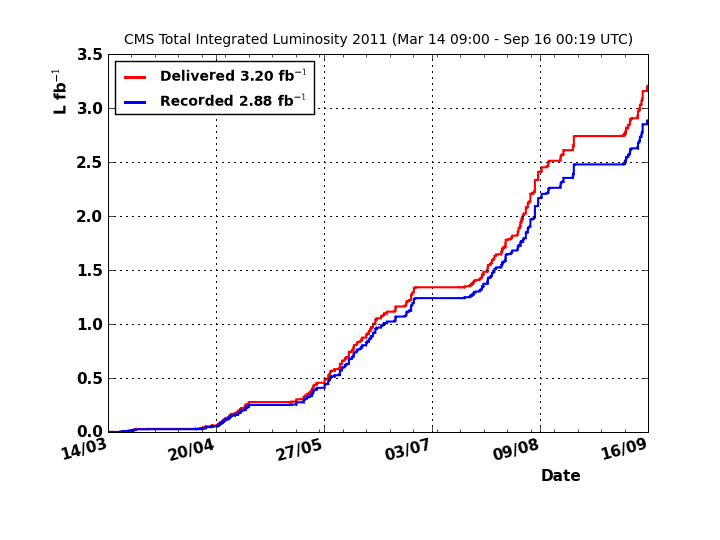
\includegraphics[width=\textwidth]{Integrated_Luminosity.png}
\caption{The integrated luminosity vs time delivered to (red) and recorded by
(blue) CMS during stable beams at $\sqrt{s} = 7 \unit{TeV}$.}
\end{center}
\label{fig:intlumi}
\end{figure}

This analysis uses $1.1 \unit{fb^{-1}}$ of data at $\sqrt{s} = 7 \unit{TeV}$ taken from 
March to June 2011. This corresponds to the data set used for the International
Europhysics Conference in High Energy Physics in July 2011. Only data certified 
by the physics validation team is included in the data set. The data set
contains the following:

\begin{itemize}
\item /PhotonHad/Run2011A-May10ReReco-v1/AOD %(Run 160404 - 163817) 
\item /PhotonHad/Run2011A-PromptReco-v4/AOD %(Run 165071 - 168437)
\item /PhotonHad/Run2011A-PromptReco-v5/AOD %(Run 170053 - 171106)
\end{itemize}

The data is split into Primary Datasets each with different trigger
requirements. PhotonHad is one such Primary Dataset. \\

%Re-processing of the data is performed periodically to ensure that data
%reconstructed using a much older version of the software is not analysed
%together with the most recent data reconstructed with the latest software
%version. The May10ReReco above is one such re-processing. 
The software version used to reconstruct the data is CMSSW\_4\_2\_3\_patch2. 
CMSSW is the standard CMS reconstruction software. The reconstruction involves 
building jets, electrons, photons and other physics objects form the raw energy 
deposits in the detector.

\section{Monte Carlo Samples}
\label{sec:Monte_Carlo_Samples}

The Monte Carlo samples used in this analysis are listed in Appendix A. The 
Monte Carlo samples are generated using Pythia 6 \cite{pythia6} or Madgraph
\cite{madgraph} with Tune Z2 (based on CTECQ6 parton distribution functions 
\cite{tuneZ2}). GEANT \cite{geant} is used for the detector simulation. \\

Pile-up is simulated in the Monte Carlo samples however the MC does not
reproduce the vertex mutiplicity distribution seen in the data. To correctly
simulate pile-up the MC is re-weighted to reproduce the number of vertices
distribution seen in the data. Figure \ref{fig:nVertices} shows the distribution
of number of vertices in the data and MC. Figure \ref{fig:reweighted} shows the
number of vertices distribution in the MC after reweighting compared to the data
to show that the correct distribution has been produced. Table \ref{tab:factors}
gives the re-weighting factors for each number of vertices. \\

\begin{figure}
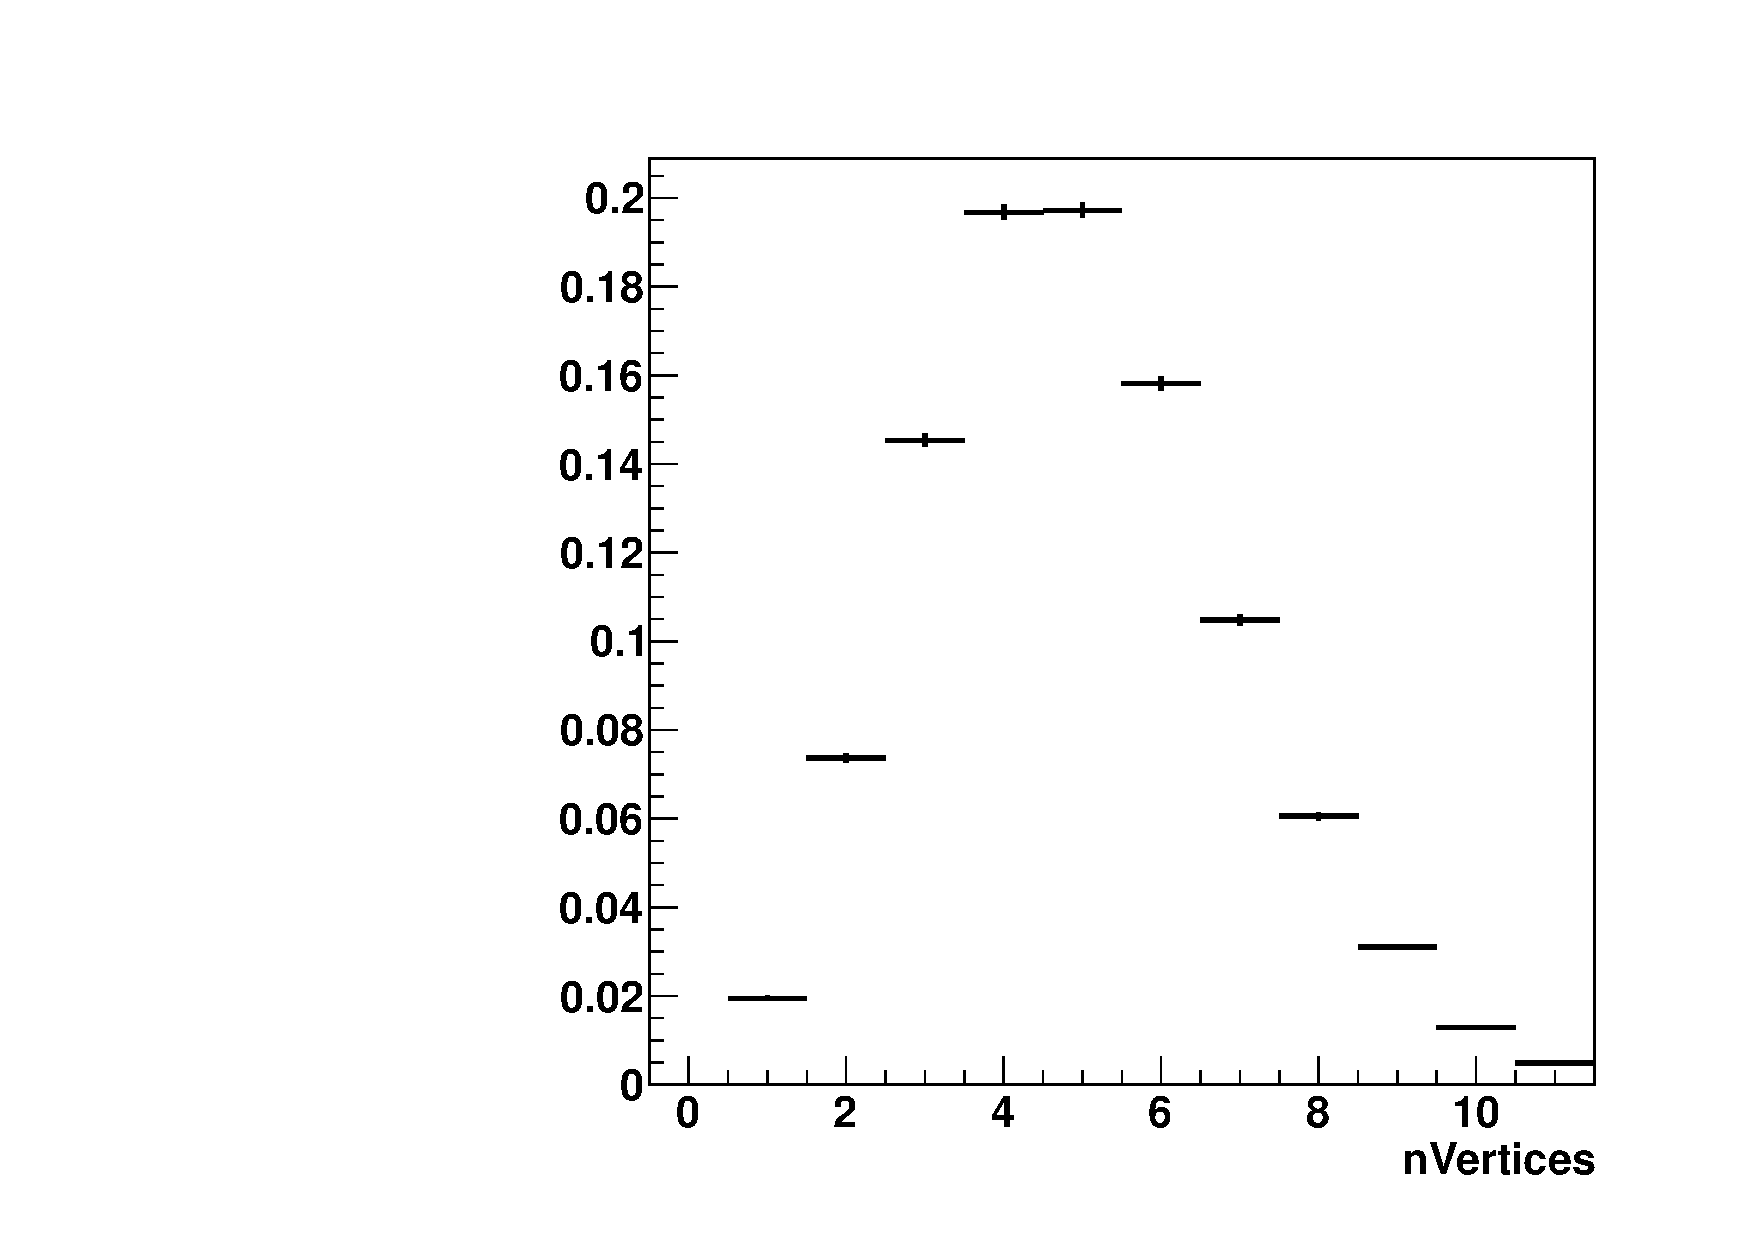
\includegraphics[width=0.5\textwidth]{nVertices-Data.pdf}
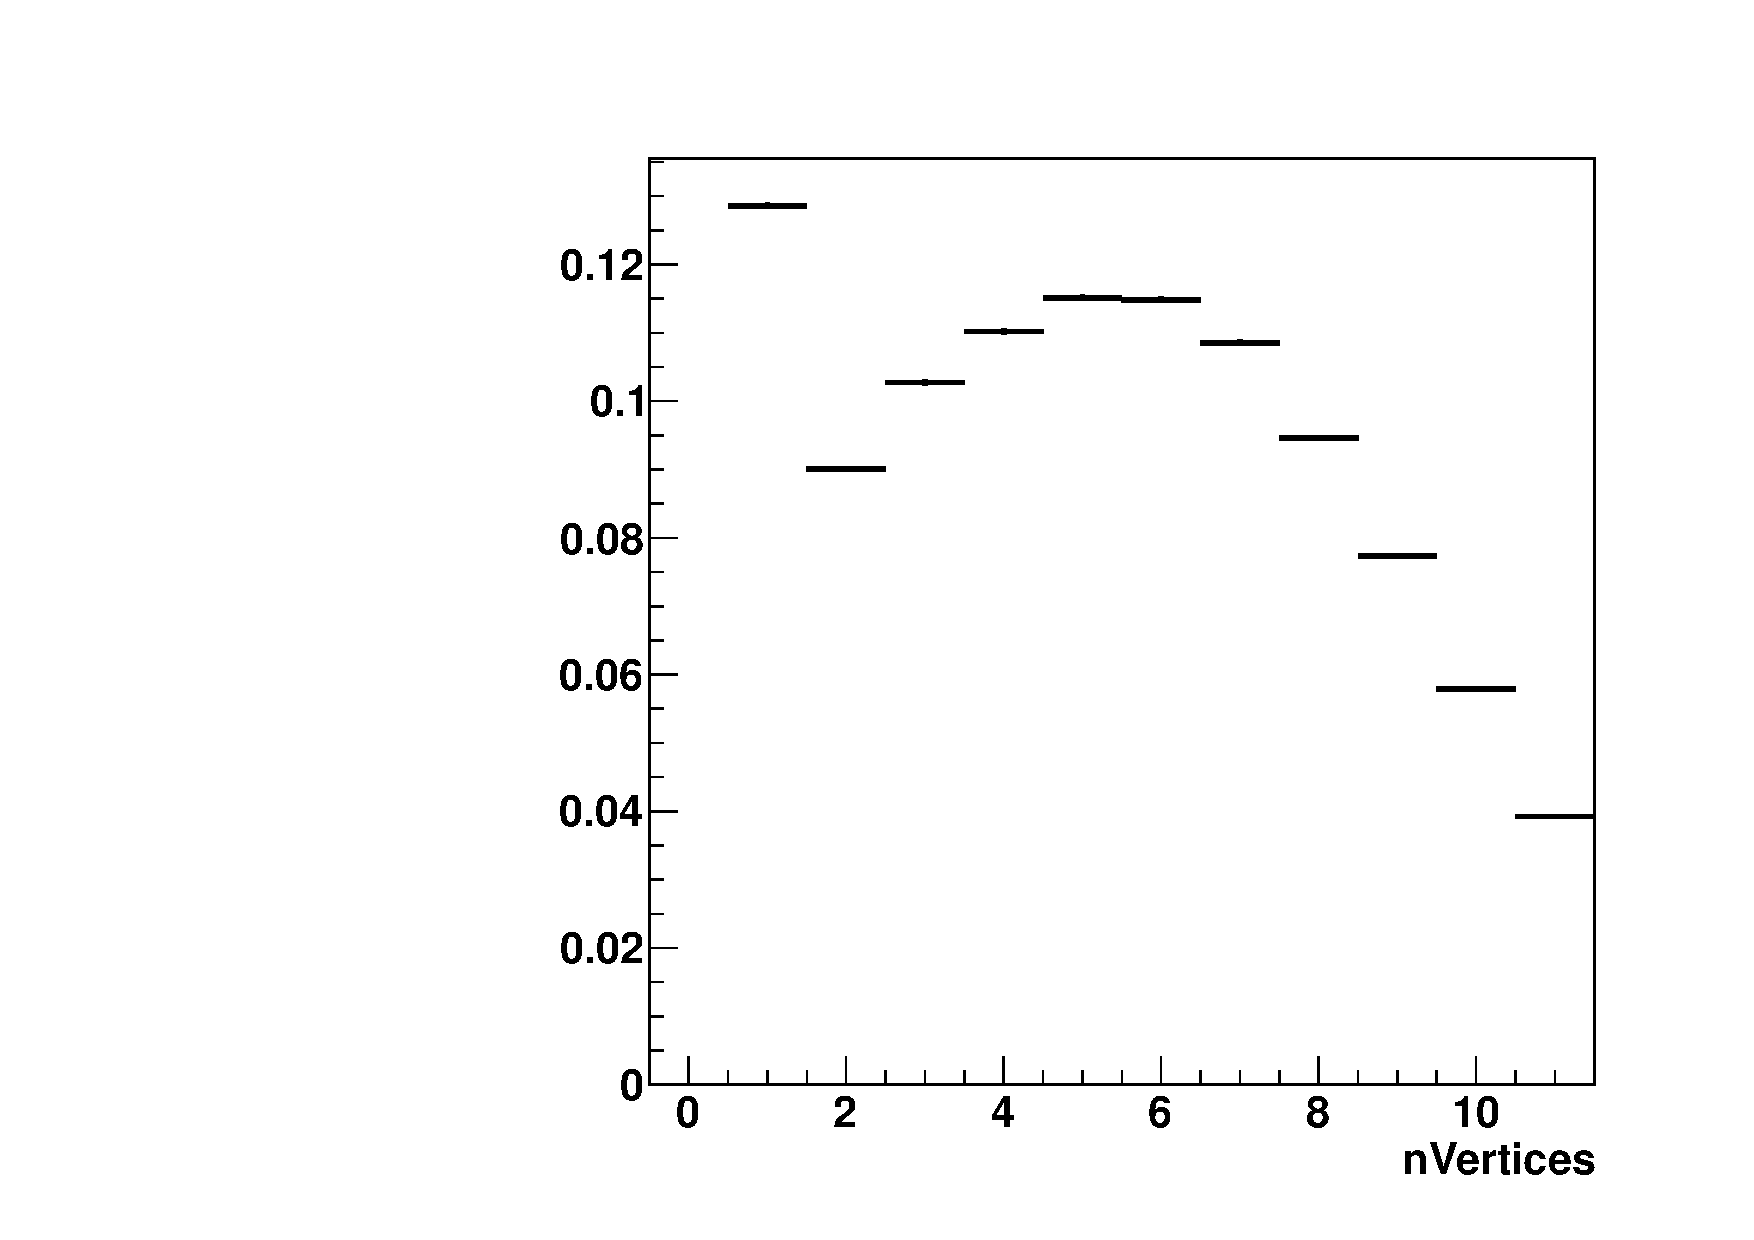
\includegraphics[width=0.5\textwidth]{nVertices-MC.pdf}
\caption{The distribution of number of vertices in the data (left) and the MC
(right).}
\label{fig:nVertices}
\end{figure}

\begin{figure}
\begin{center}
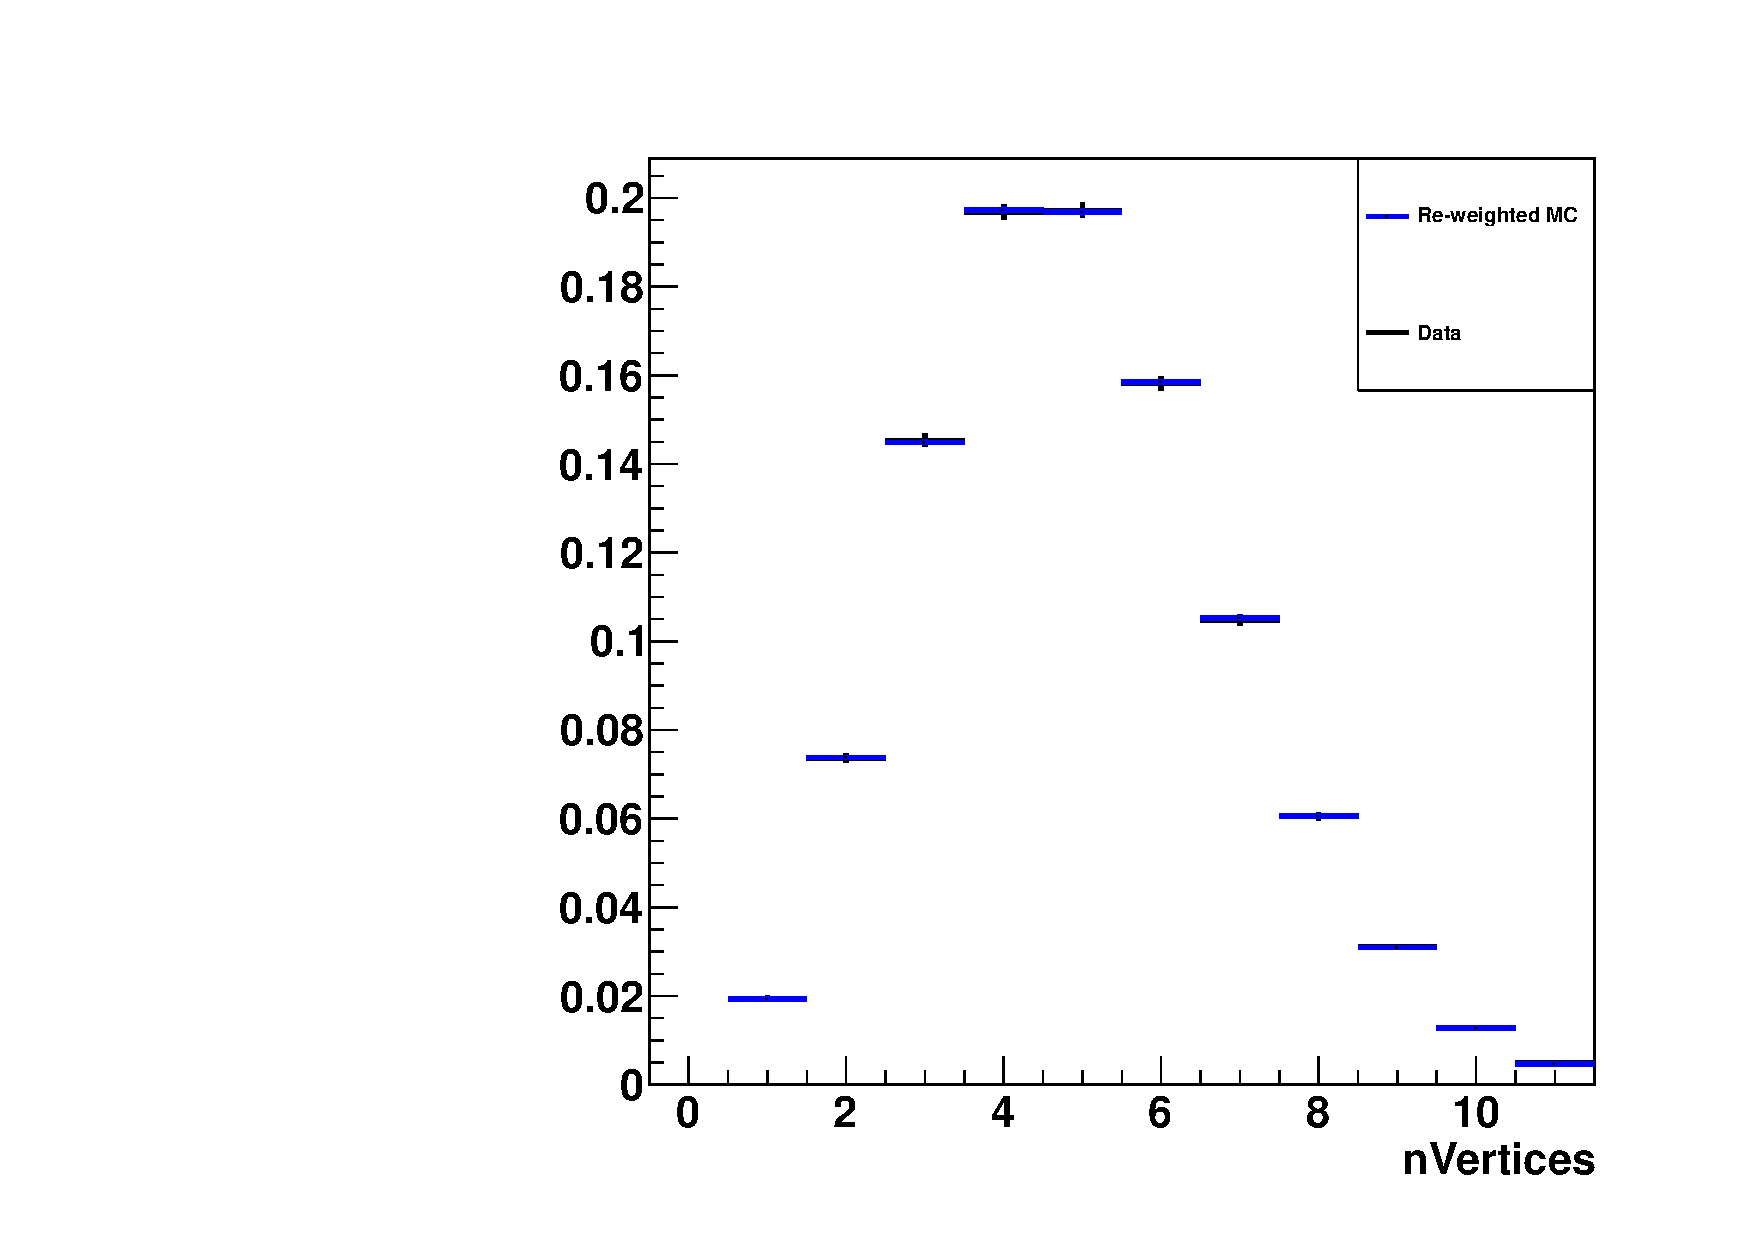
\includegraphics[width=0.5\textwidth]{nVertices-MC-reweighted.pdf}
\end{center}
\caption{The distribution of number of vertices in the MC after reweighting
(blue) compared to the data (black).}
\label{fig:reweighted}
\end{figure}

\begin{table}
\begin{center}
{\scriptsize
\begin{tabular}{|l|c|c|c|c|c|c|c|c|c|c|c|c|c|}
\hline
nVertices & 1 & 2 & 3 & 4 & 5 & 6 & 7 & 8 & 9 & 10 & 11 & 12 \\
\hline
Weight & 0.15 & 0.82 & 1.41 & 1.79 & 1.71 & 1.38 & 0.97 & 0.64 & 0.40 & 0.22 &
0.12 & 0.04 \\
\hline
\end{tabular}}
\end{center}
\caption{Re-weighting factors to be applied to the MC to correctly reproduce the
number of vertices distribution in the data.}
\label{tab:factors}
\end{table}

Figure \ref{fig:Data_vs_MC} shows plots of a few key variables to show how
accurately the Monte Carlo models the data. The Monte Carlo prediction is
good for $\HT$, but the $\MET$ distribution is not accurately predicted by the 
Monte Carlo. \\

\begin{figure}
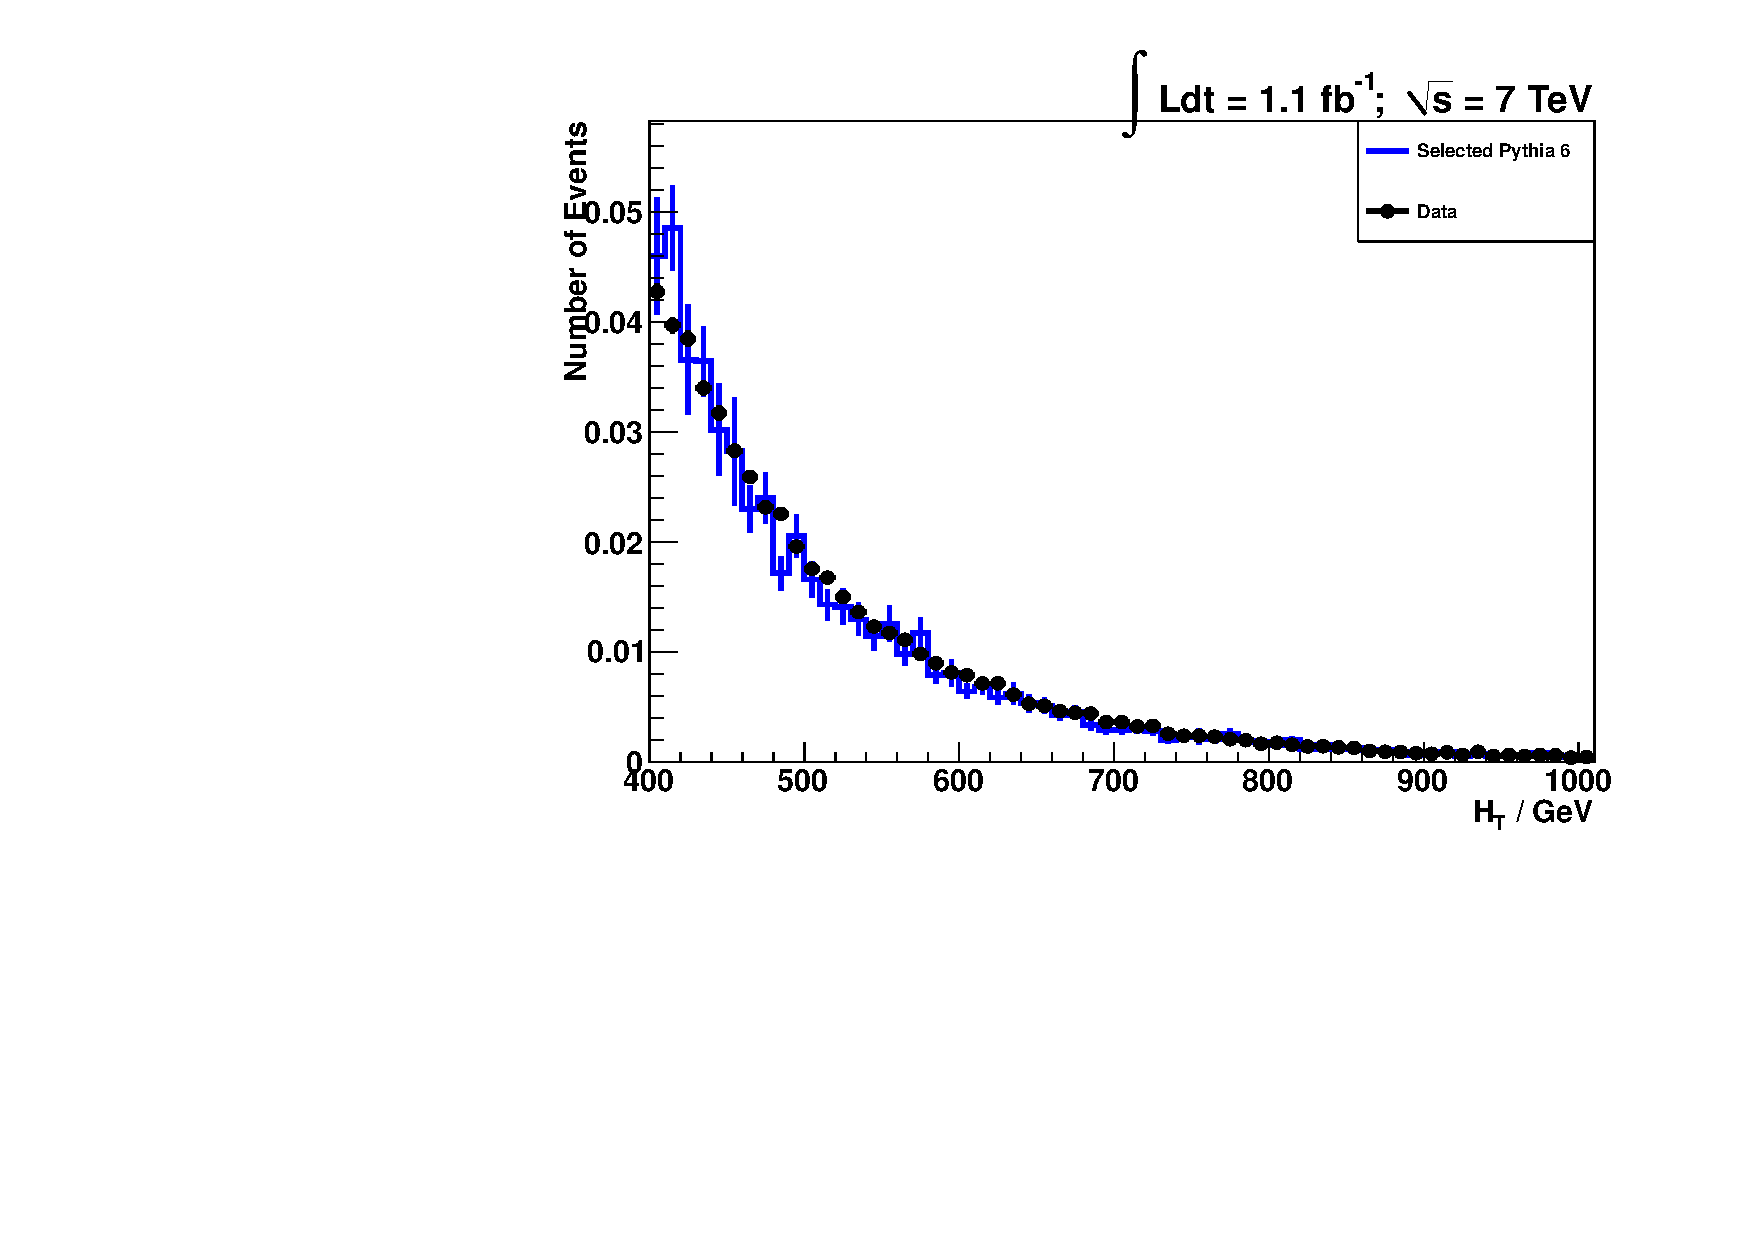
\includegraphics[width=0.5\textwidth]{HT_all.pdf}
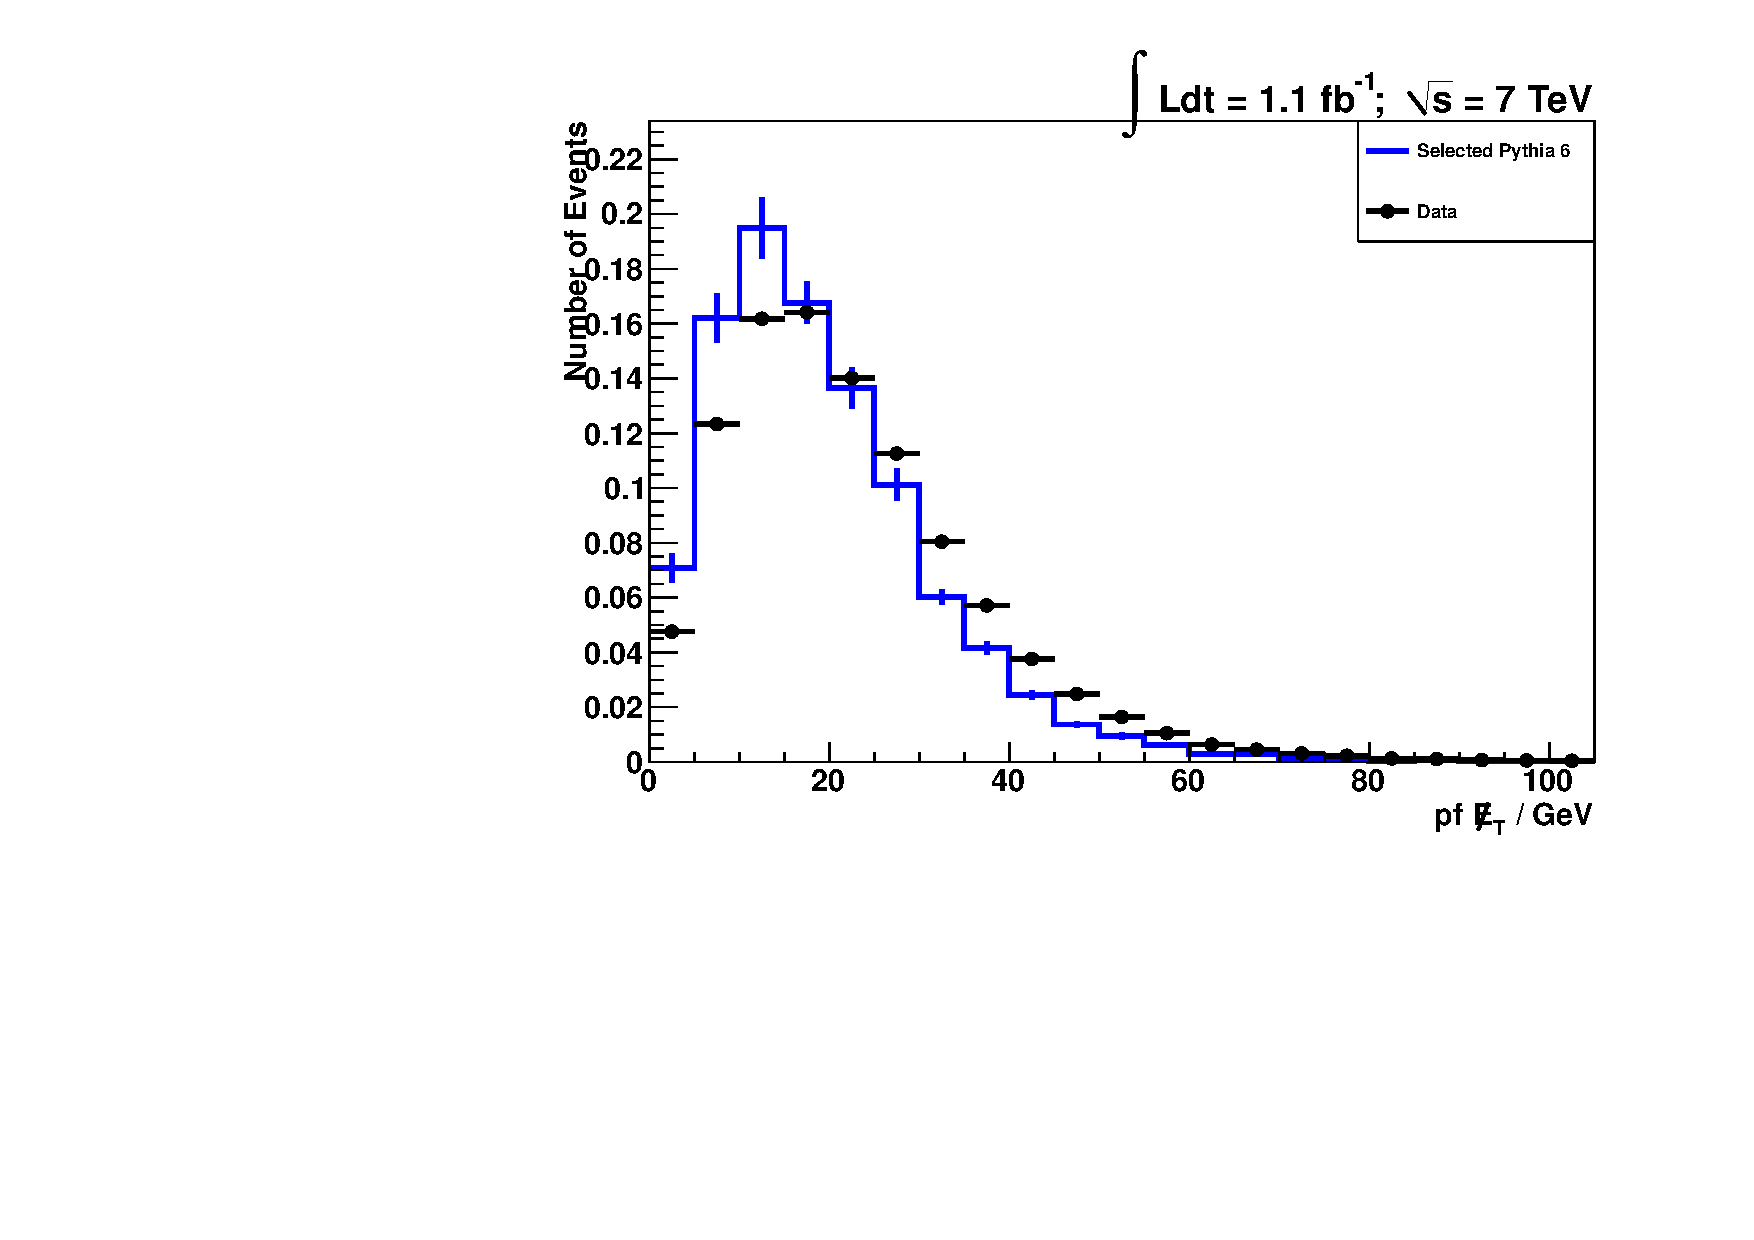
\includegraphics[width=0.5\textwidth]{pfMET_all.pdf}
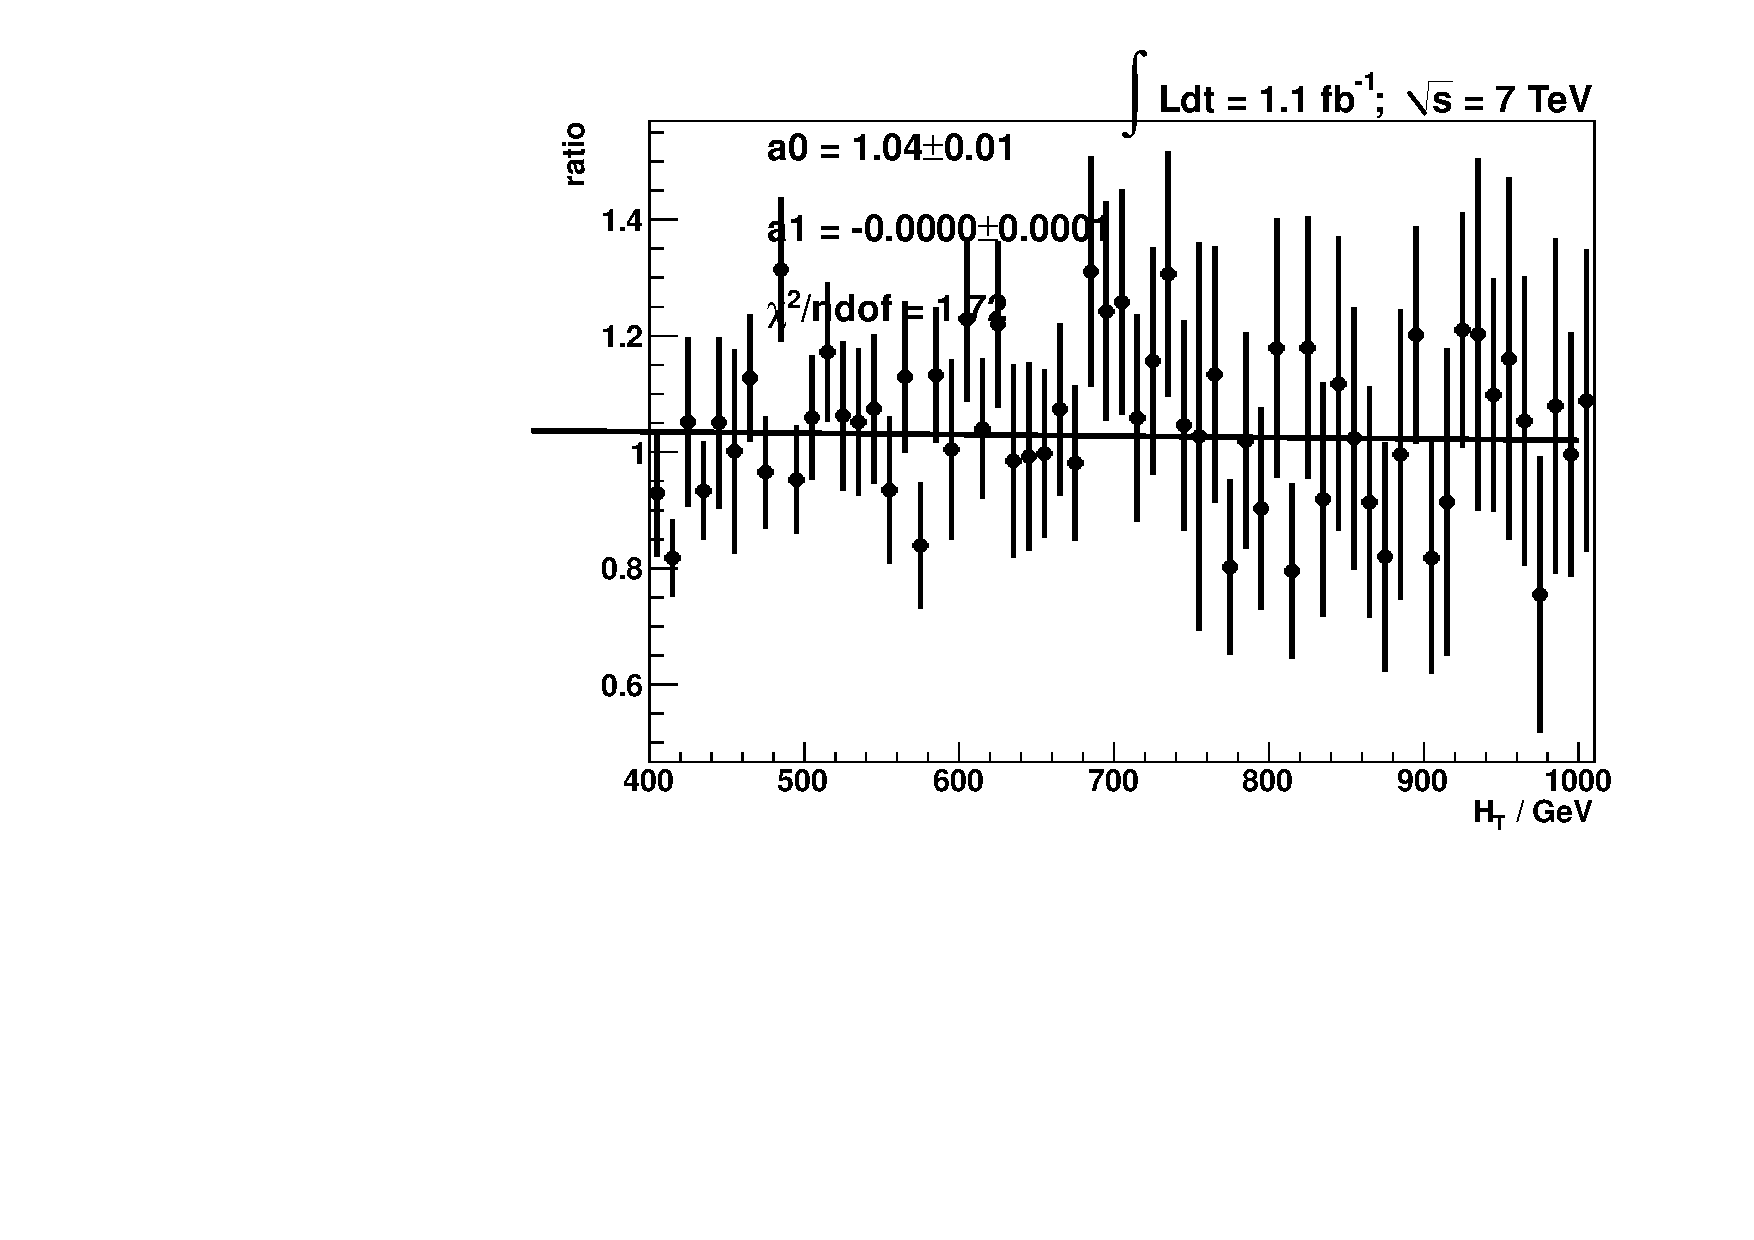
\includegraphics[width=0.5\textwidth]{HT_all_ratio.pdf}
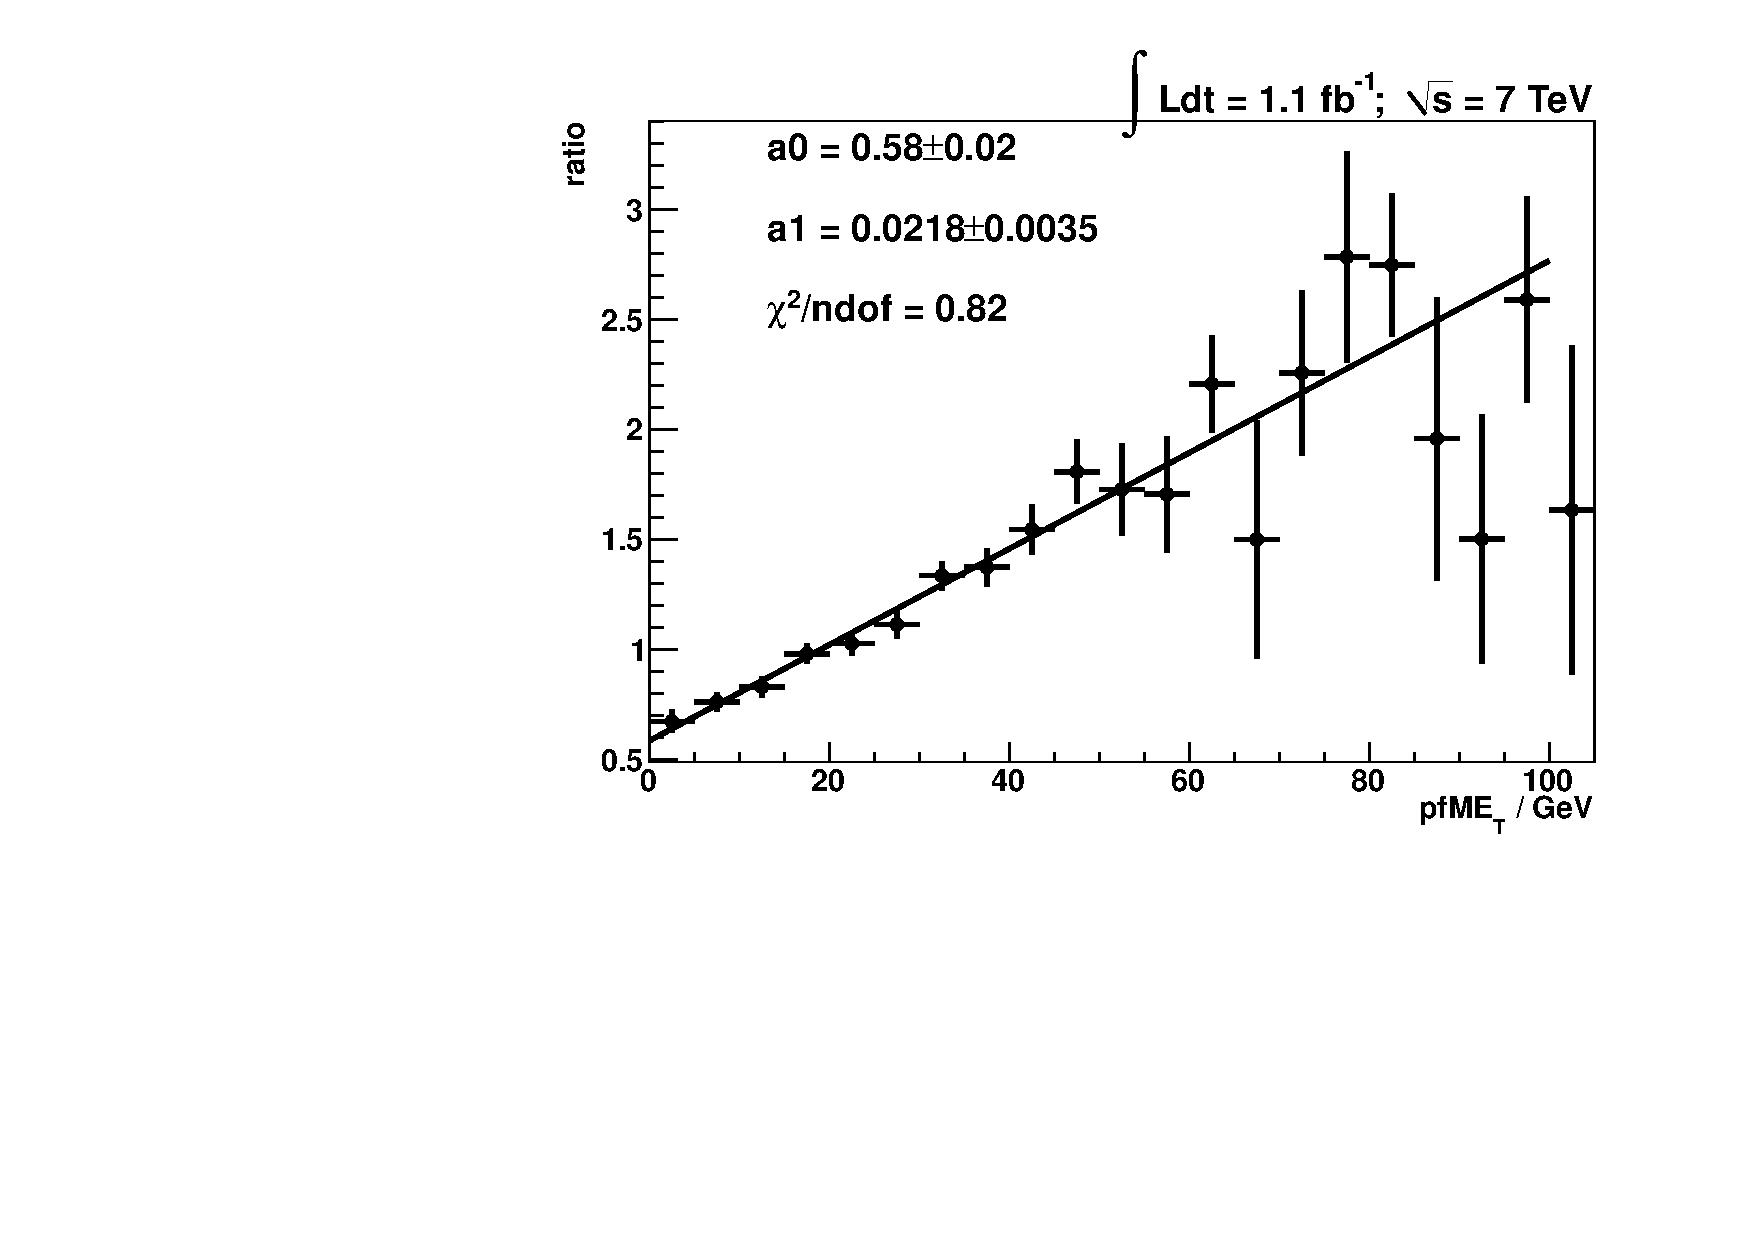
\includegraphics[width=0.5\textwidth]{pfMET_all_ratio.pdf}
\caption{Plots of $\HT$ and MET in data and Monte Carlo to show how accurately
the Monte Carlo models the data. Ratio plots of data/MC are shown below.}
\label{fig:Data_vs_MC}
\end{figure}

%\begin{figure}
%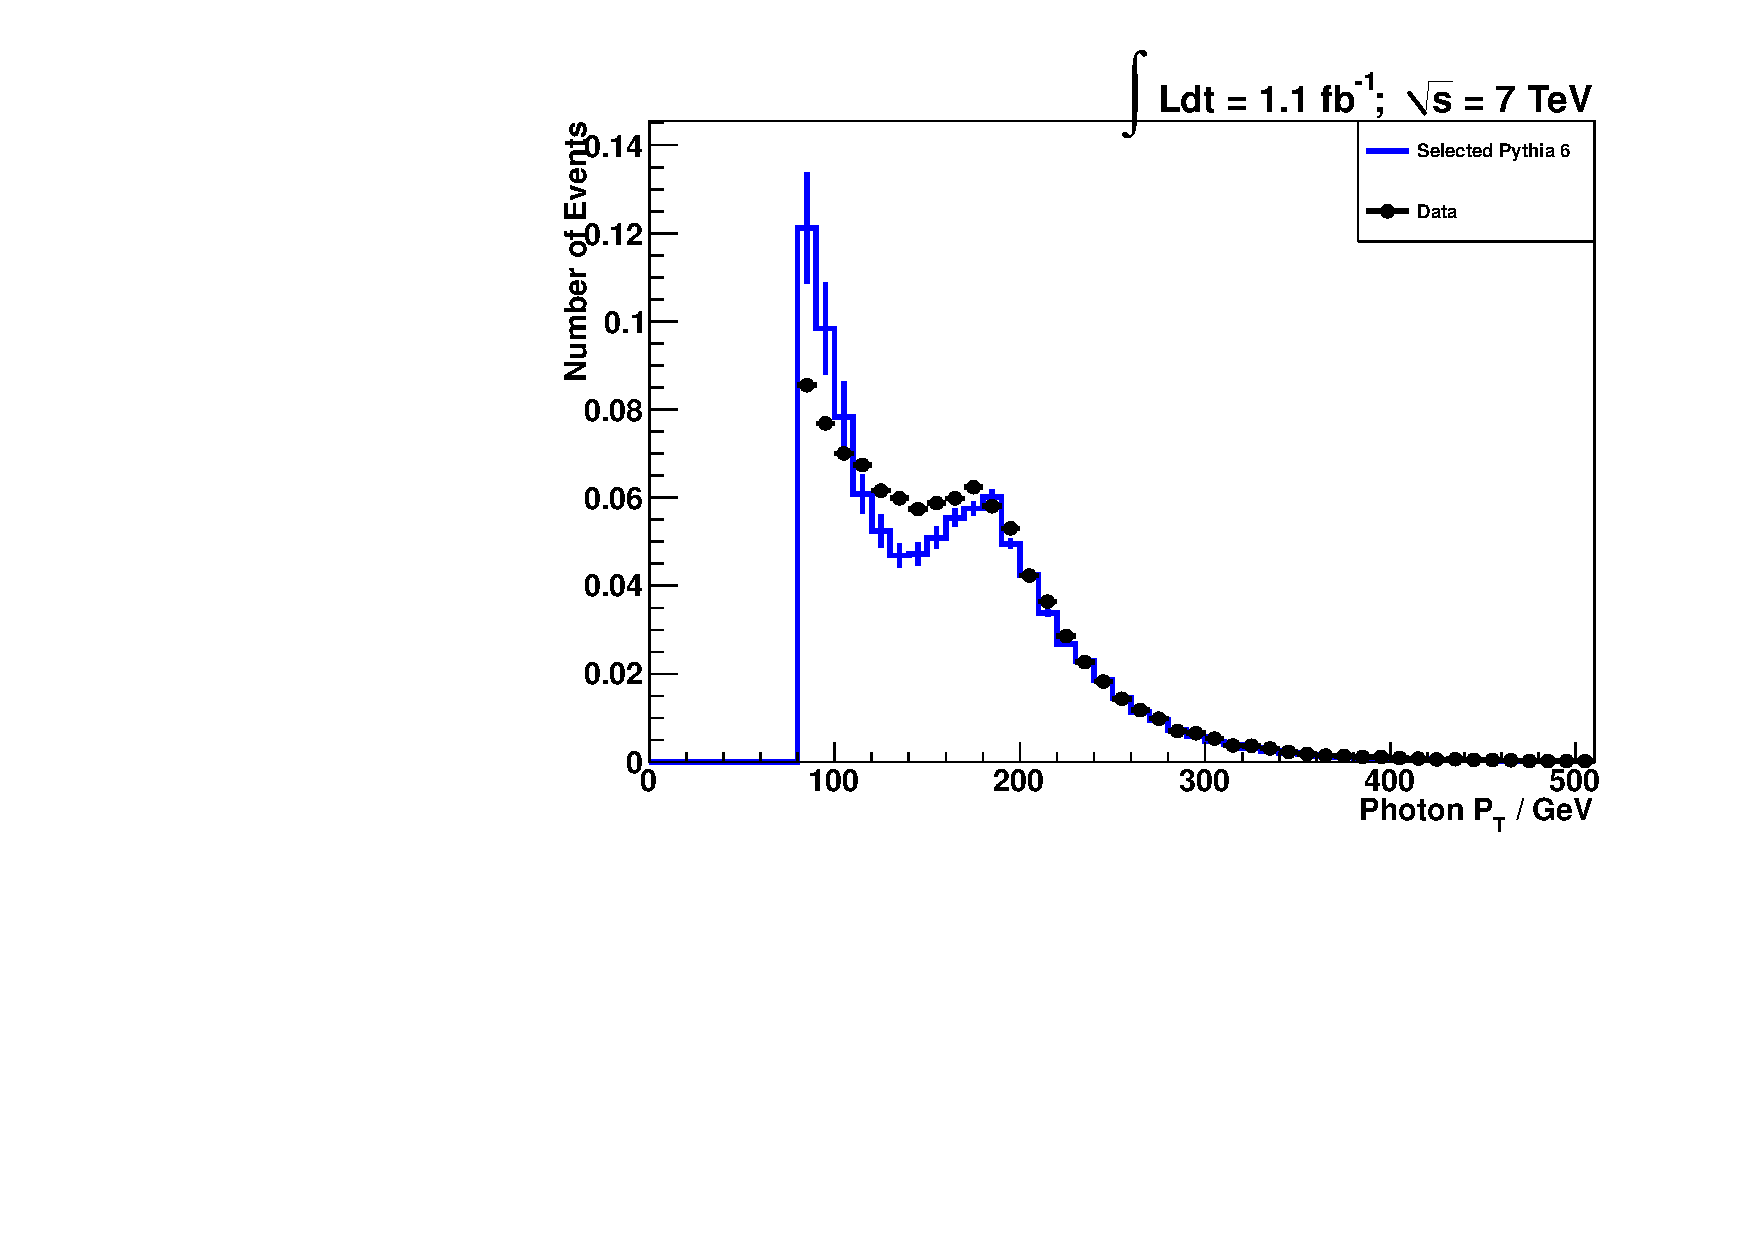
\includegraphics[width=0.5\textwidth]{PhotonPt_all.pdf}
%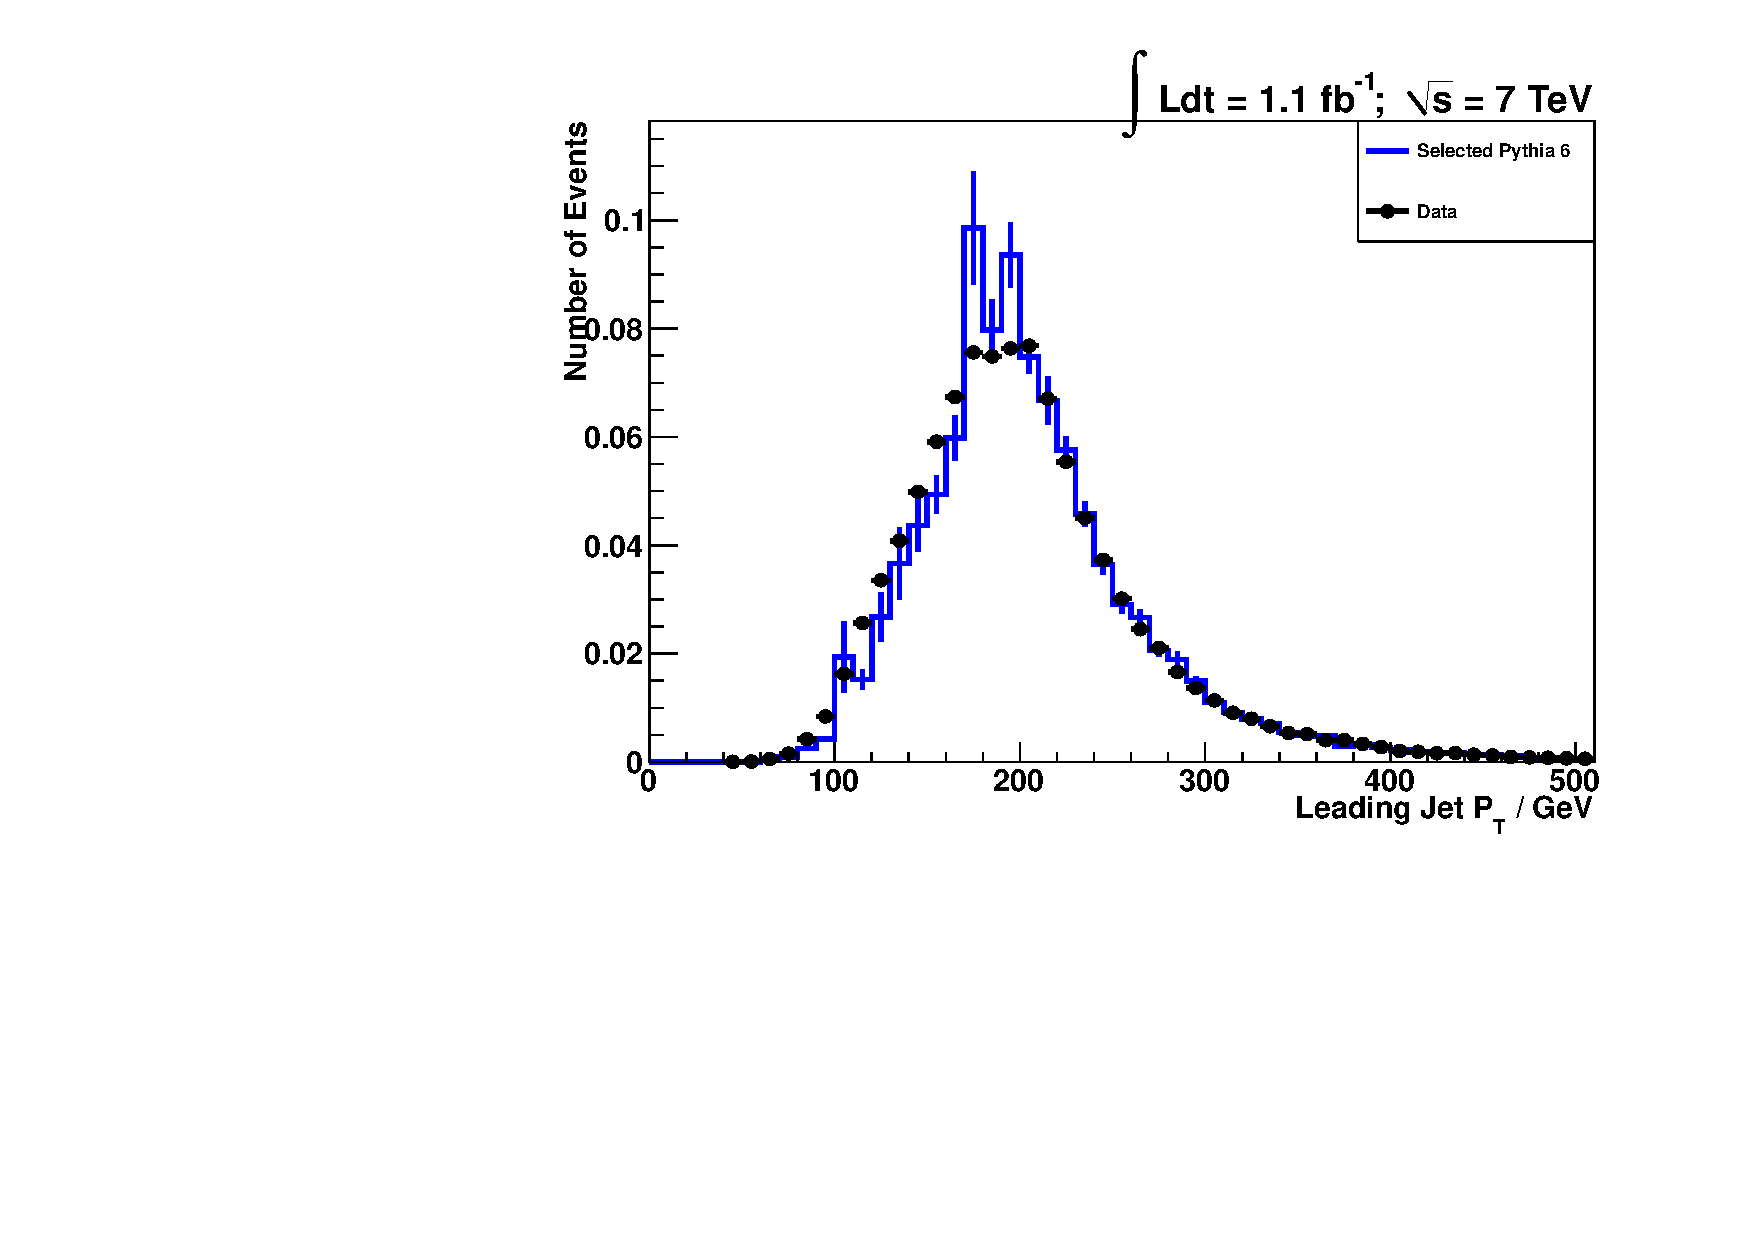
\includegraphics[width=0.5\textwidth]{Jet1Pt_all.pdf}
%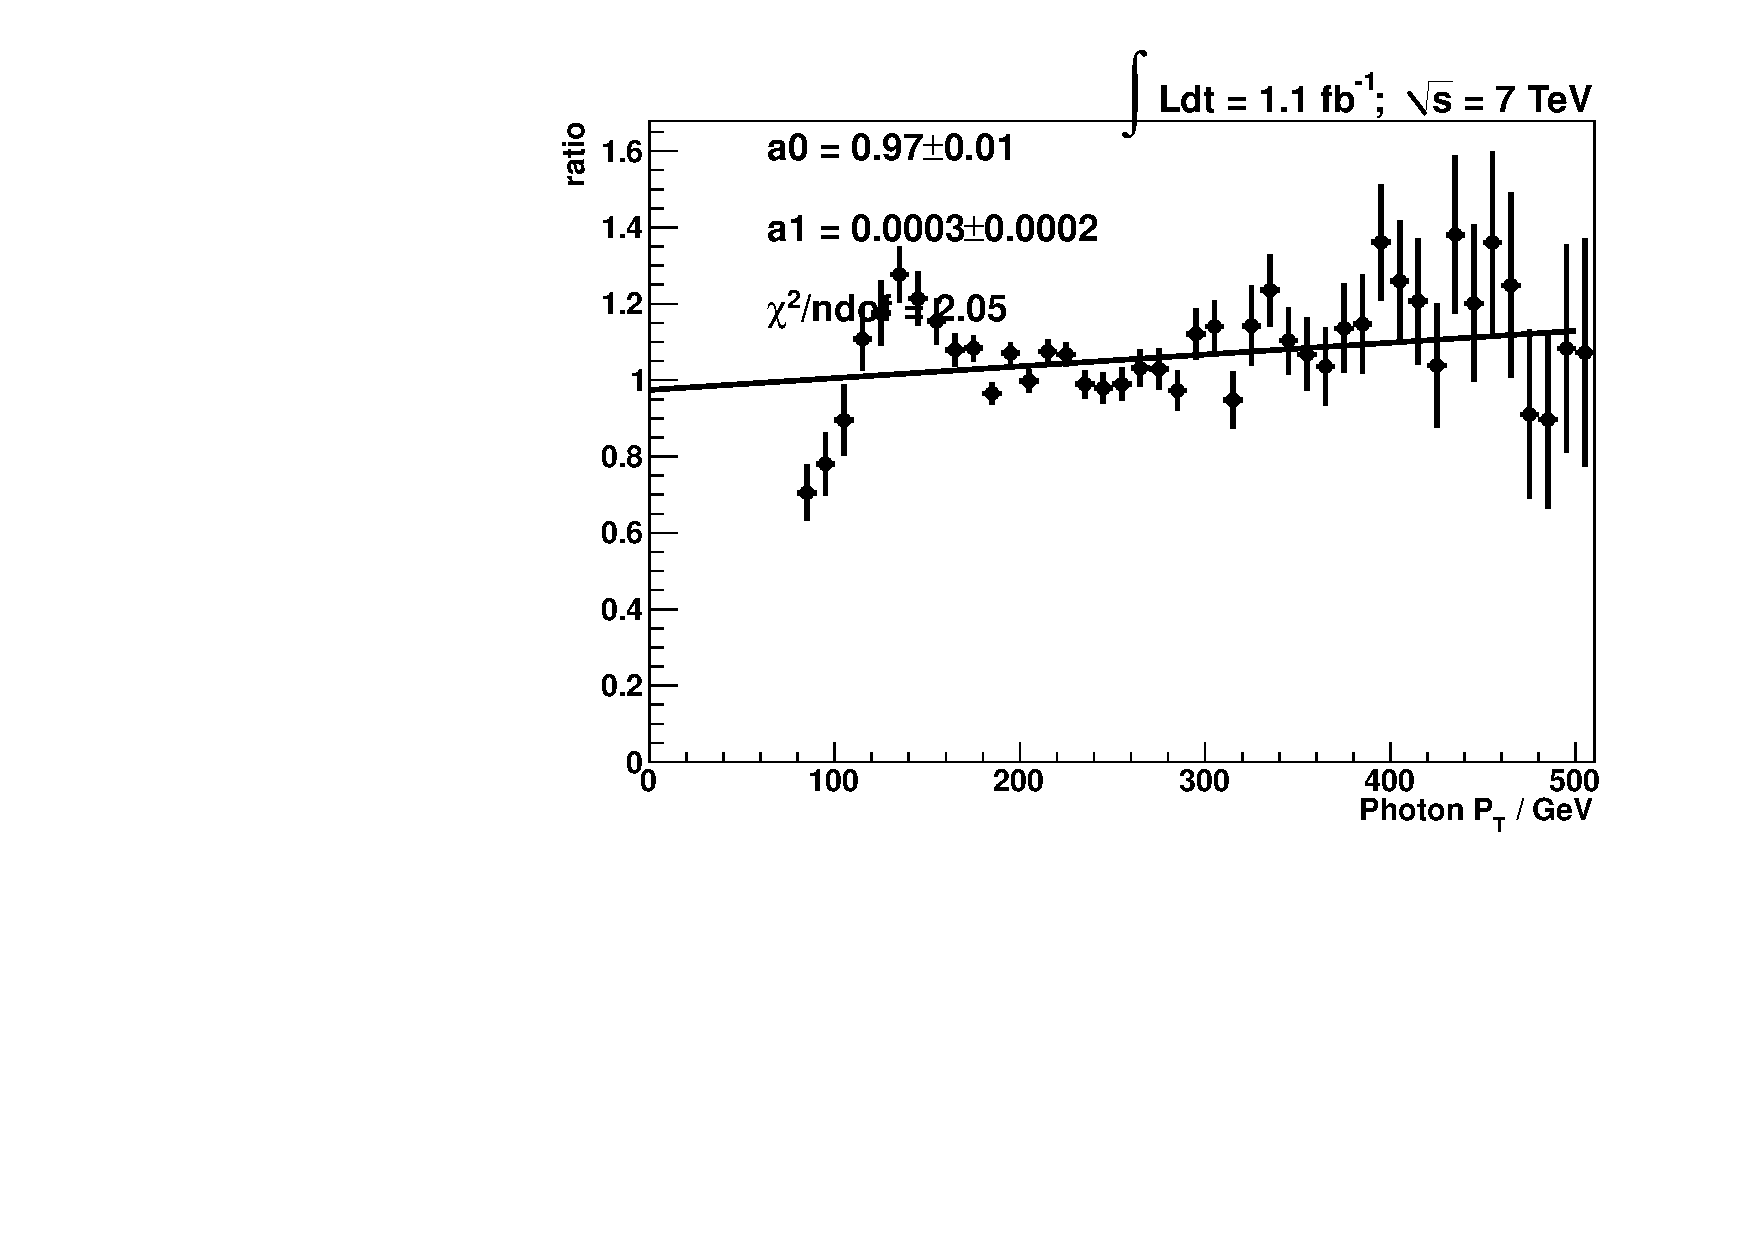
\includegraphics[width=0.5\textwidth]{PhotonPt_all_ratio.pdf}
%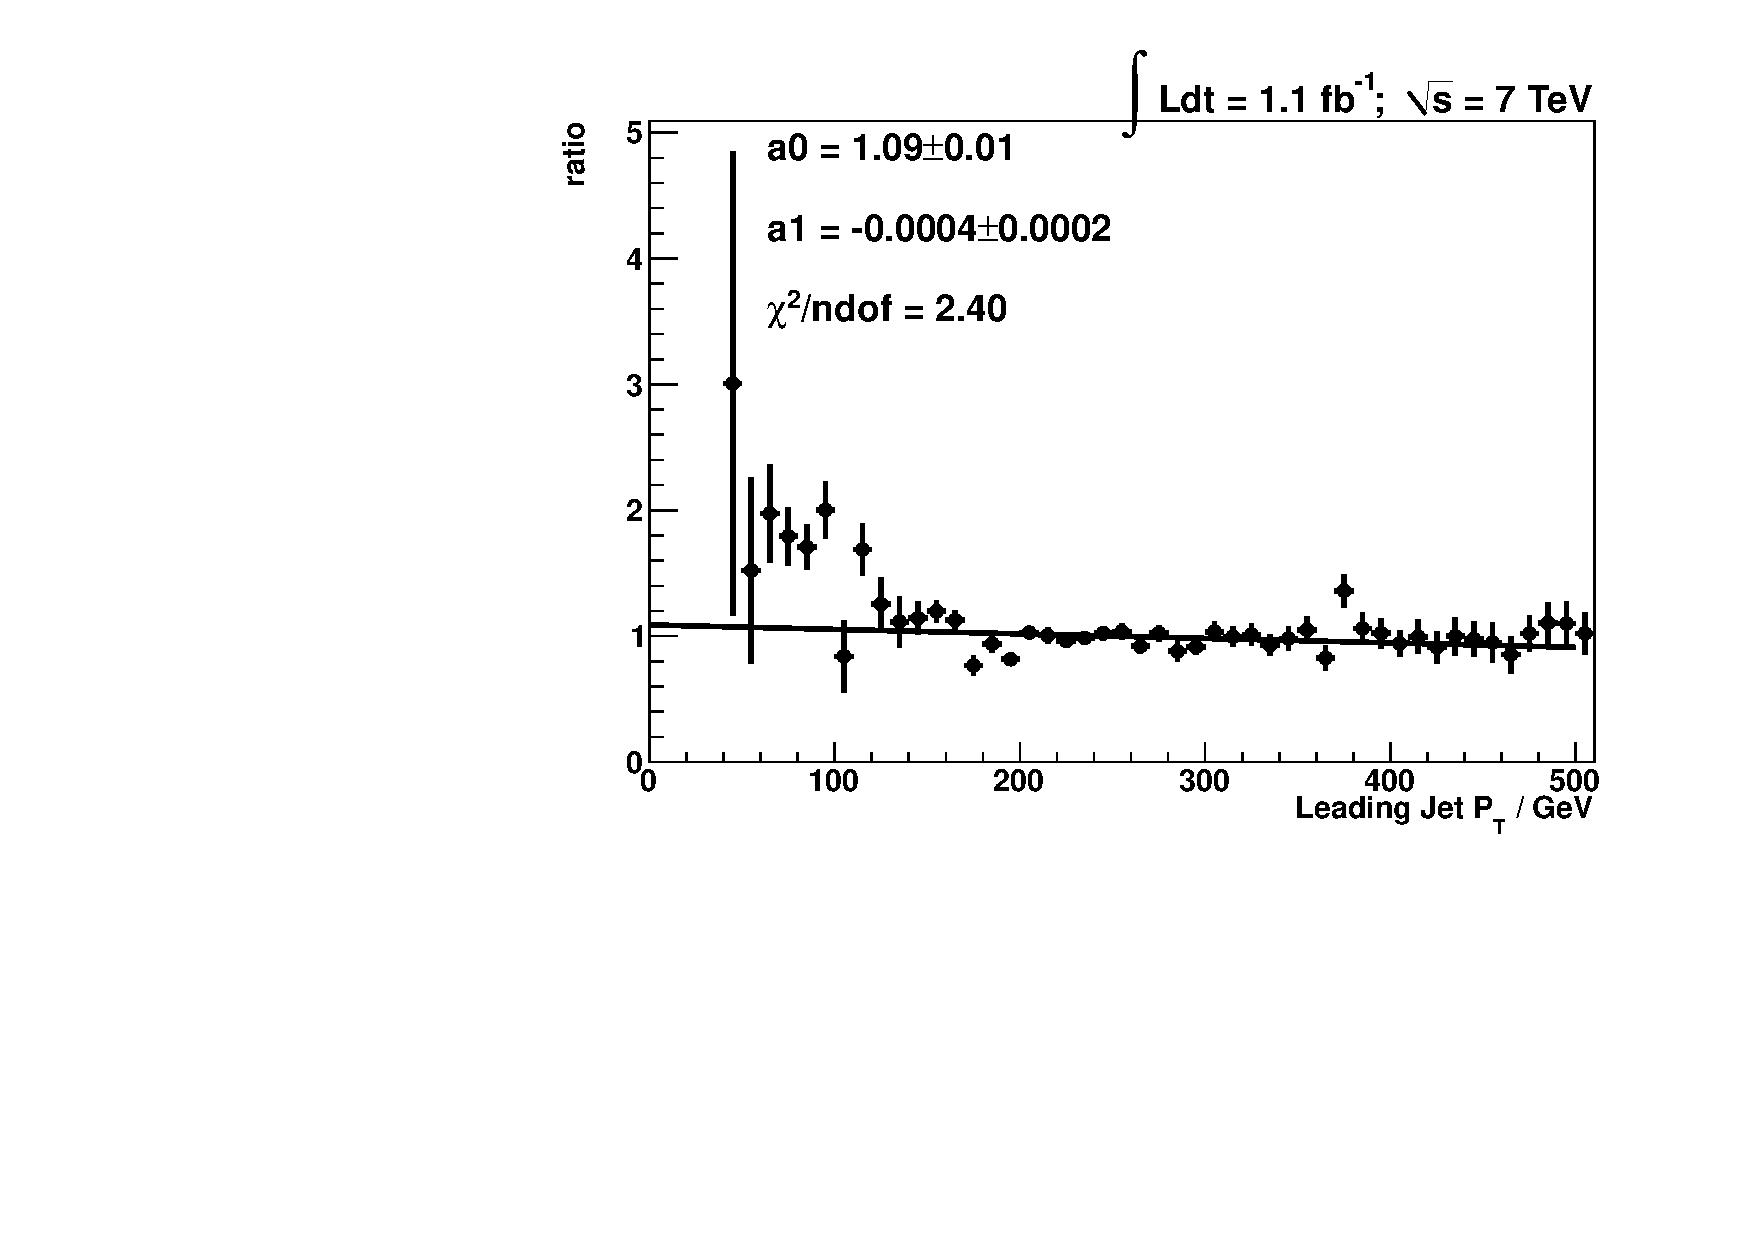
\includegraphics[width=0.5\textwidth]{Jet1Pt_all_ratio.pdf}
%\caption{Plots of photon $\pT$ and leading jet $\pT$ in data and Monte Carlo to
%show how accurately the Monte Carlo models the data. Ratio plots of data/MC are
%shown below.}
%\label{fig:Data_vs_MC}
%\end{figure}

Since the background estimation (see Section \ref{sec:QCD_Background}) is 
largely data-driven the dependence of the result on Monte Carlo is limited. \\

\section{Trigger}

With a soft QCD cross-section of $\sim1\unit{mb}$ and a luminosity of $\sim 
10^{33}\unit{cm^{-1}s^{-1}}$ $(1\unit{nb^{-1}s^{-1}})$ the event rate is $\sim
10^{6} \unit{Hz}$. 
Most of these are uninteresting events and the DAQ bandwidth limits the rate at 
which data can be read out. The goal of the trigger is to select the interesting 
events to read out. \\

There are two components to the trigger: Level 1 and HLT. The Level 1 trigger
sits in a cavern next to the CMS detector. It takes ``trigger primitives'' such
as crystal energy sums calculated by on-detector hardware which are transferred 
by optical link from the CMS detector. The goal is to reduce the rate to $\sim 
10\unit{Hz}$. Those events which pass the Level 1 trigger are fully read out and
unpacked by the HLT. The HLT is run on a farm of computers in a room above the 
CMS detector. It reconstructs physics objects and makes decisions based on the 
presence and quality of these to further reduce the rate to $\sim 200\unit{Hz}$. \\

Based on the properties of strong production GMSB, a photon + $\HT$ trigger 
is ideal for this search. Table \ref{tab:Triggers} shows a list of all the 
photon + $\HT$ triggers in the 2011 data with the corresponding L1 seed and the
rate at $10^{33}\unit{cm^{-2}s^{-1}}$. \\

\begin{table}
\begin{center}
\begin{tabular}{|l|c|c|}
\hline
 & L1 seed & Rate at $10^{33}\unit{cm^{-2}s^{-1}}$ \\
\hline
HLT\_Photon60\_CaloIdL\_HT200 & L1\_SingleEG20 & (pre-scaled) \\
HLT\_Photon70\_CaloIdL\_HT200 & L1\_SingleEG20 & (pre-scaled) \\
HLT\_Photon70\_CaloIdL\_HT300 & L1\_SingleEG20 & $4\unit{Hz}$ \\
HLT\_Photon70\_CaloIdL\_HT350 & L1\_SingleEG20 & $2.5\unit{Hz}$ \\
\hline
\end{tabular}
\end{center}
\caption{A table of the photon and $\HT$ triggers available in the 2011 data
along with the corresponding L1 seed and rate at $10^{33}\unit{cm^{-2}s^{-1}}$.}
\label{tab:Triggers}
\end{table}

As the luminosity has increased more stringent trigger requirements have been 
necessary to keep the data rate manageable. If the rate of a trigger becomes too
high, the trigger must be pre-scaled. This means that only every nth event which
fires the trigger is read out where n is the prescale factor. Figure 
\ref{fig:Trigger_vs_Run_Number} shows the run ranges over which the various 
photon and jet triggers are in the trigger menu and when they become pre-scaled.
\\

\begin{figure}
\begin{center}
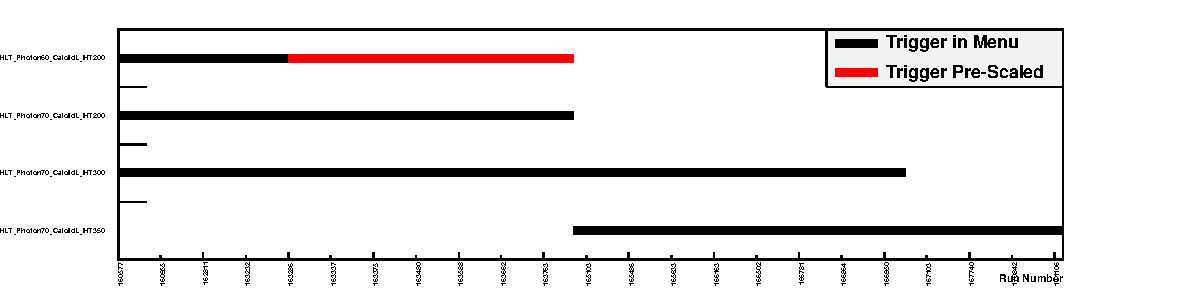
\includegraphics[width=\textwidth]{Trigger_vs_Run_Number.pdf}
\end{center}
\caption{The run range over which photon and jet triggers are in the menu and
when they are pre-scaled.}
\label{fig:Trigger_vs_Run_Number}
\end{figure}

The efficiency of a trigger is evaluated with respect to a lower threshold
trigger. Data ranges are selected such that the two triggers are both in the
menu and both unprescaled. The triggers, A and B, are identical except that B 
has a higher threshold in variable x than A. To find out the efficiency of B:

\begin{enumerate}
\item Select events that pass A.
\item Plot the distribution of x to get histogram h\_A.
\item Select events that also pass B.
\item Plot the distribution of x in these events to get histogram h\_B.
\item Divide h\_B by h\_A, bin-by-bin to get the efficiency vs x.
\end{enumerate}

In this case the variable x is $\HT$ or photon $\pT$. The efficiency curve tells
us where to put the off-line cut in x such that the trigger is fully efficient.
\\

The efficiency is determined over the run ranges where the trigger overlaps with
one of a lower threshold (see Figure \ref{fig:Trigger_vs_Run_Number}). Figure 
\ref{fig:Trigger_Efficiency} shows the trigger efficiency against $\HT$ and 
photon $\pT$.

\begin{figure}
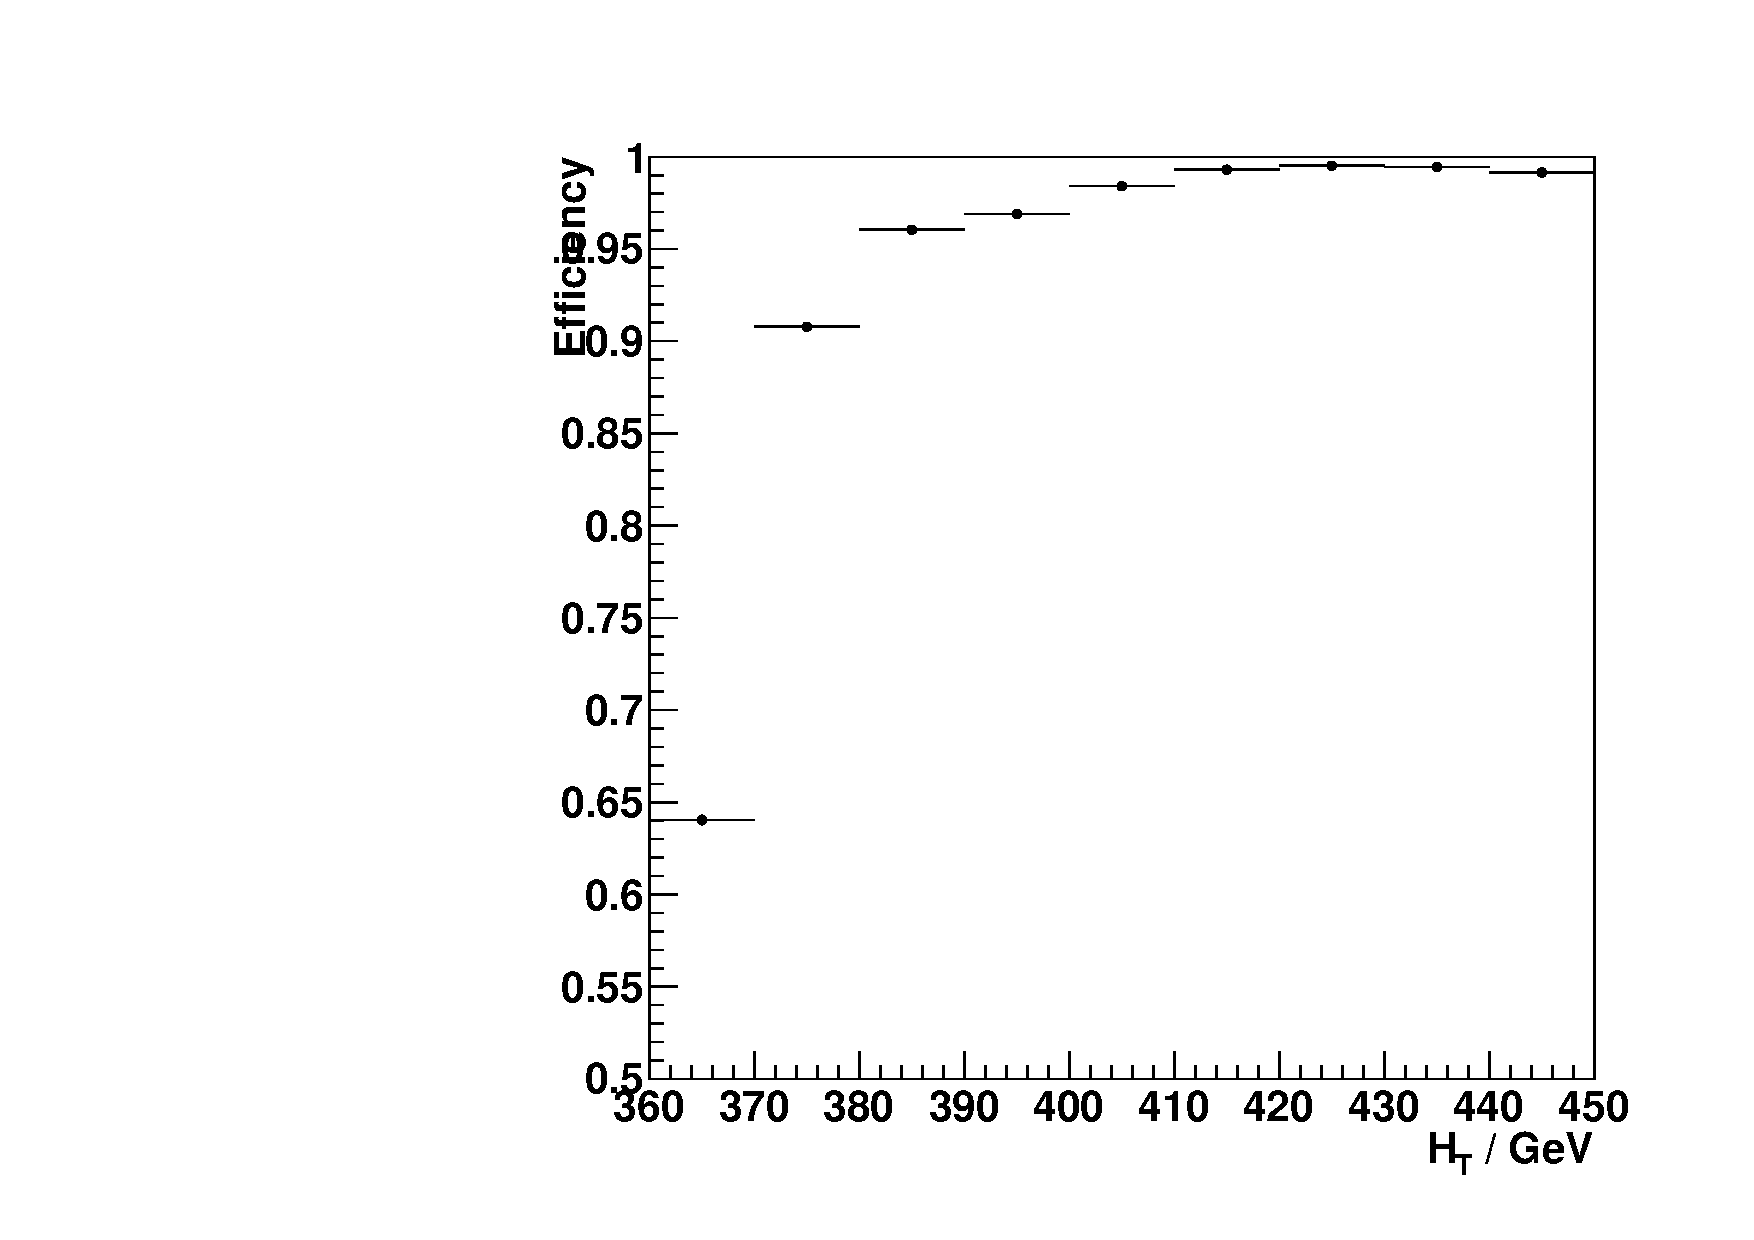
\includegraphics[width=0.5\textwidth]{Trigger_Efficiency_vs_HT_zoomed.pdf}
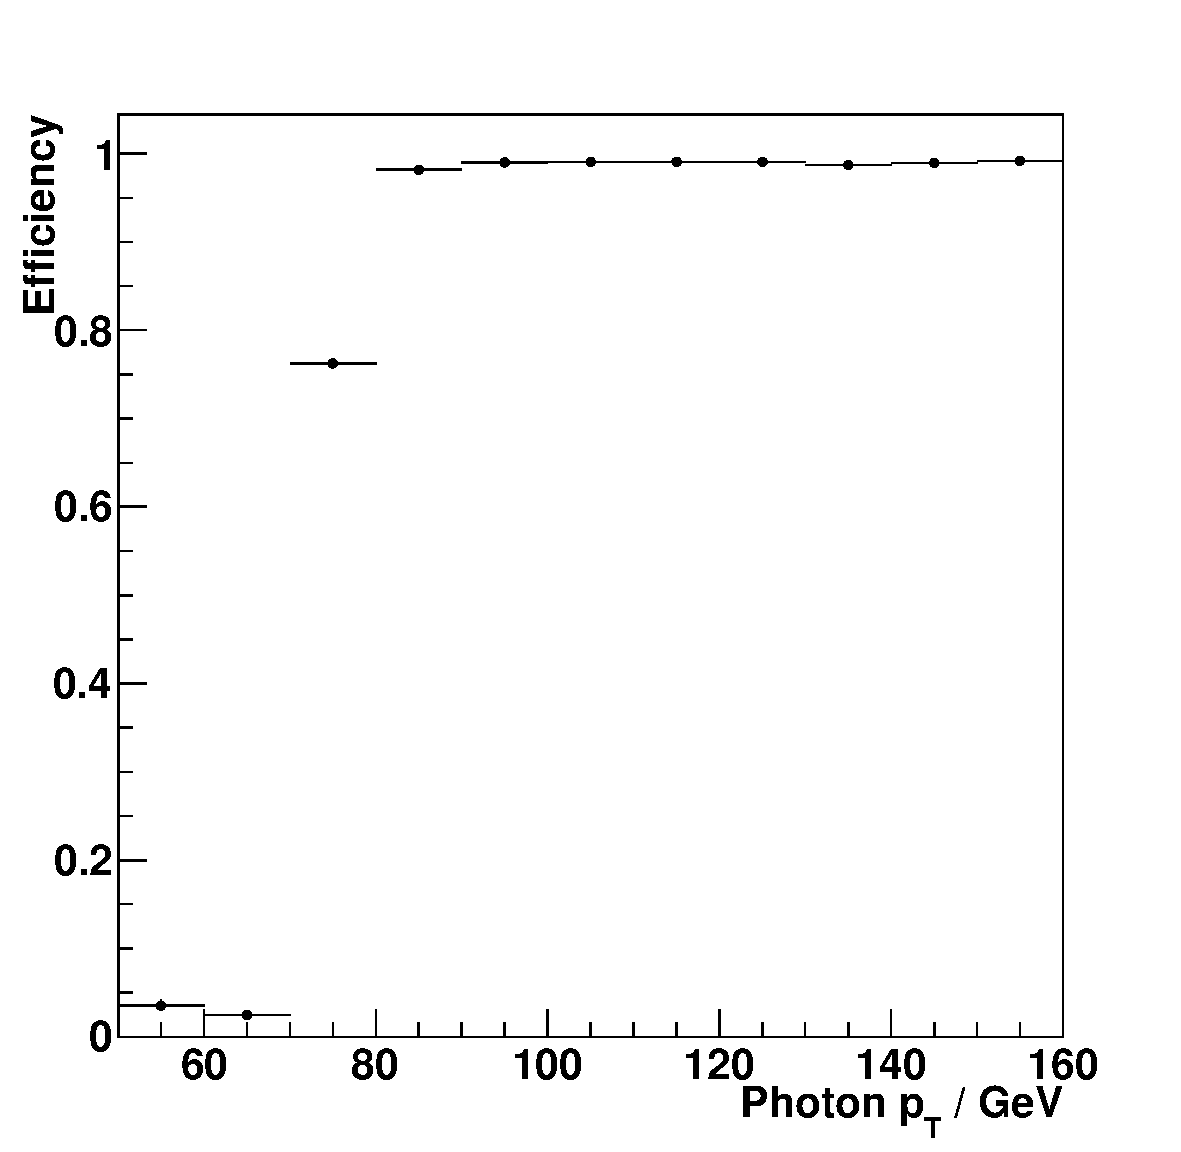
\includegraphics[width=0.5\textwidth]{Trigger_Efficiency_vs_PhotonPt.pdf}
\caption{The trigger efficiency vs $\HT$ (left) and vs photon $\pT$ (right)
relative to a lower threshold trigger.}
\label{fig:Trigger_Efficiency}
\end{figure}

\section{Photon Selection}

Photons are selected based on variables such as isolation and shower shape which
are designed to select prompt photons over fakes from jets. The photon 
reconstruction is described in detail in Section \ref{sec:photon_recontruction}. 
The cut values on each of the photon selection varaibles are listed in Table 
\ref{tab:photoncuts}. 

\begin{table}
\begin{center}
\begin{tabular}{|c|c|c|}
\hline
ECAL isolation & $4.2 + 0.006\pT$ \\
\hline
HCAL isolation & $2.2 + 0.0025\pT$ \\
\hline
Track isolation & $2.0 + 0.001\pT$ \\
\hline
H/E & 0.05 \\
\hline
Shower Shape & 0.013 \\
\hline
No Pixel Seed & True \\
\hline
\end{tabular}
\end{center}
\caption{The photon selection cuts.}
\label{tab:photoncuts}
\end{table}

\section{Jet Selection}

Two jets with $\pT > 80 \unit{GeV}$ and $|\eta| < 2.5$ are required. The $\eta$
threshold corresponds to the tracker boundary. The $\pT$ threshold should be
chosen as high as possible to reject background, but with the signal efficiency
close to 100\%. Figure \ref{fig:Jet_Threshold} shows the signal efficiency and 
the background rejection as a function of the jet $\pT$ threshold. 

\begin{figure}
\begin{center}
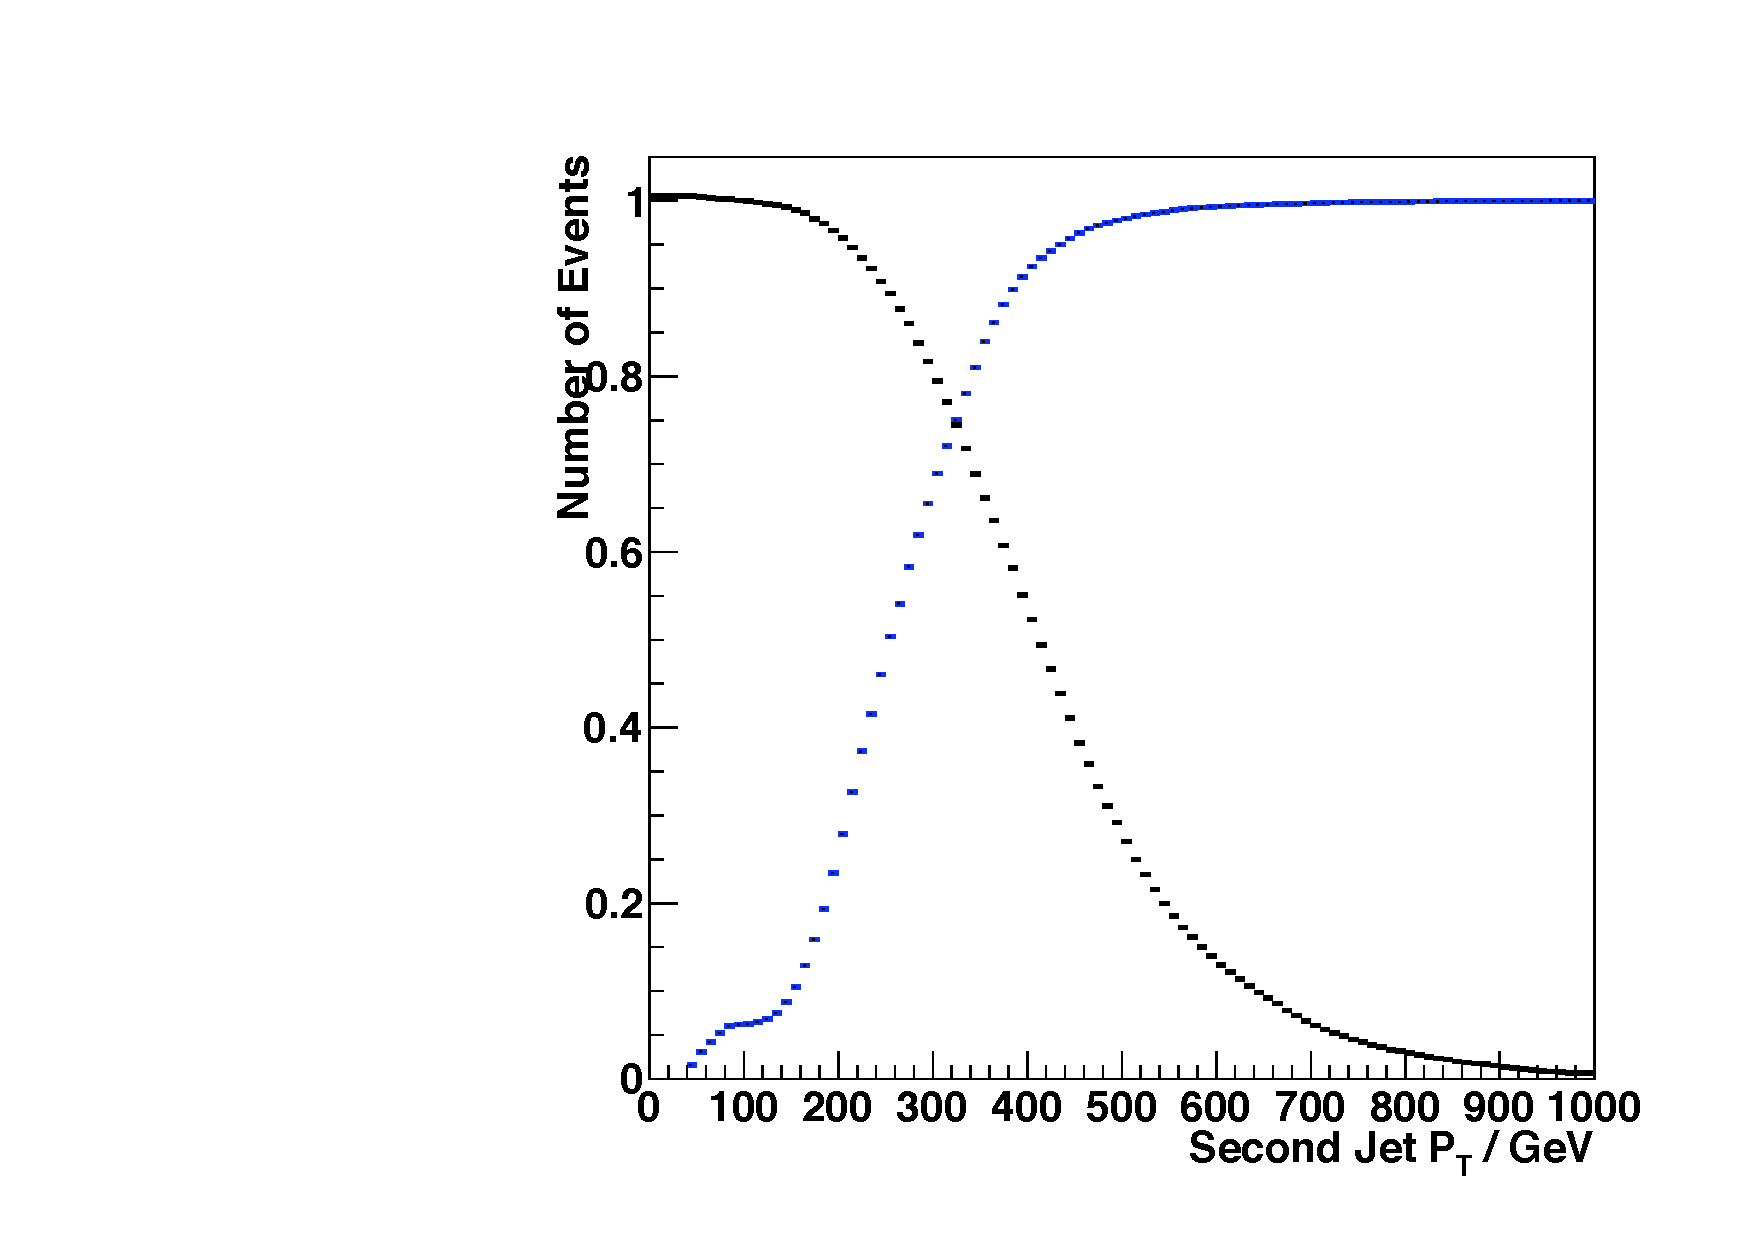
\includegraphics[width=0.7\textwidth]{Jet_Threshold.pdf}
\end{center}
\caption{A plot of the efficiency of the signal (black) and the background
rejection (blue) as a function of the jet $\pT$ threshold.}
\label{fig:Jet_Threshold}
\end{figure}

\section{Missing Transverse Energy}

By conservation of momentum, the sum of the momenta of all the final state
particles in a collision is equal to the sum of the momenta of all the inital
state particles. The initial longitudinal momentum of the colliding partons is
unknown since the fraction of the proton momentum that each parton carries is
unknown for any individual event. However, the initial transverse momentum is
known to be zero so the final transverse momentum must also be to zero. \\

Events with small missing transverse energy are to be expected because the 
detectors are not perfect: they have a finite resolution. In addition to this
there is a resolution from fluctuations inherent in the hadronic shower. Missing
transverse energy from these source are expected to be gaussian distributed in x
and y. Large missing transverse energy can come from undetected particles e.g. 
neutrinos or detector imperfections e.g. dead cells. \\

The missing transverse energy is calculated using the sum of the transverse
momentum of the reconstructed particles. For high energy photons and jets, the 
most accurate determination of the momentum comes from the energy measurement in
the calorimeters. The transverse energy of an energy deposit E is calculated as 
in Equation \ref{eq:et}. The missing transverse energy is calculated as the
negative sum of the transverse energies of all the energy deposits (Equation
\ref{eq:met}). \\

\begin{equation}
\overrightarrow{\ET} = E\sin{\theta}\cos{\phi}\vec{x} + E\sin{\theta}\sin{\phi}\vec{y}
\label{eq:et}
\end{equation}

\begin{equation}
\overrightarrow{\MET} = - \Sigma \overrightarrow{\ET} \unit{cm}
\label{eq:met}
\end{equation}

Motivated by SUSY, this search is based on missing energy. In R-parity
conserving SUSY models events have decay chains ending in the Lightest 
Supersymmetric Particle (LSP) which goes undetected and hence shows up as 
missing transverse energy. In contrast, QCD events (which are the dominant 
background) have only fake missing energy due to detector imperfections. \\

\section{Event Selection}

The event selection criteria are listed below. 

\begin{itemize}
\item Noise Cleaning
\item $\HT > 400 \unit{GeV}$
\item $\geq 2$ jets
\item $\geq 1$ photon
\item $\MET > 50 \unit{GeV}$
\end{itemize}

Threee types of noise cleaning are applied to the events. 
\begin{itemize}
\item {\bf Primary Vertex Selection:} Events are required to have at least one
Primary Vertex with $|z| < 24\unit{cm}$, $\mbox{nDOF} > 4$ and $\rho <
2\unit{cm}$.
\item {\bf HCAL Noise Filter:} There are three types of HCAL noise: HPD noise, 
RBX noise and PMT window noise. HPD noise comes from the hybrid photodiodes in
the HB, HE and HO. Misallignment between the HPD electric field and the external
magnetic field can lower the flashover voltage of the HPD resulting in 
occasional cascades where all or most of the 18 channels within the HPD report
large energy deposits. RBX noise is when all or most of the 72 channels in a
Readout Box report large energies. The origin of this noise is cross-over in the
electronics where a signal causes an induced signal in neighbouring wires.
PMT window noise comes from charged particles occasionally hit an HF PMT window 
directly instead of interacting with the quartz fibres. This results in a large 
energy deposit in either a long or a short fibre without an appreciable deposit 
in the other short/long partner. The HCAL noise filter removes HCAL noise by 
vetoing on variables related to pulse shape, timing, hit multiplicity and number
of zero ADC counts.
\item {\bf ECAL Spike Cleaning:} ECAL Spikes are isolated energy deposits in 
the ECAL which do not come from EM showers. The origin of ECAL spikes is pions
going directly into the depleted region of the photodetector (without
interacting in the ECAL) making it look like there is a significant energy 
deposit in the ECAL. ECAL spikes lead to fake photons and fake MET. There are 
two properties which characterise ECAL spikes: topology and timing. ECAL spikes 
tend to be single crystal enrgy deposits in the ECAL which are often not vetoed 
by the shower shape variable. Some spikes are in time with the rest of the event 
and some are out of time. The energy varies from a few MeV to a few TeV. A 
cut of $1 - e4/e1 < 0.96$ is made to avoid ECAL Spikes. 1 - e4/e1 is the ``Swiss 
Cross'' variable in which e1 is the highest energy crystal in a 3x3 array and e4 
is the energy of the four adjacent crystals. Additional spikes with significant
energy in two adjacent crystals remained. These residual spikes are vetoed by
requiring $e2/e9 < 0.96$ and $|t| < 5\unit{ns}$, t is the timing of the signal. This 
is illustrated by Figure \ref{fig:spikes}.
\end{itemize}

\begin{figure}
\begin{center}
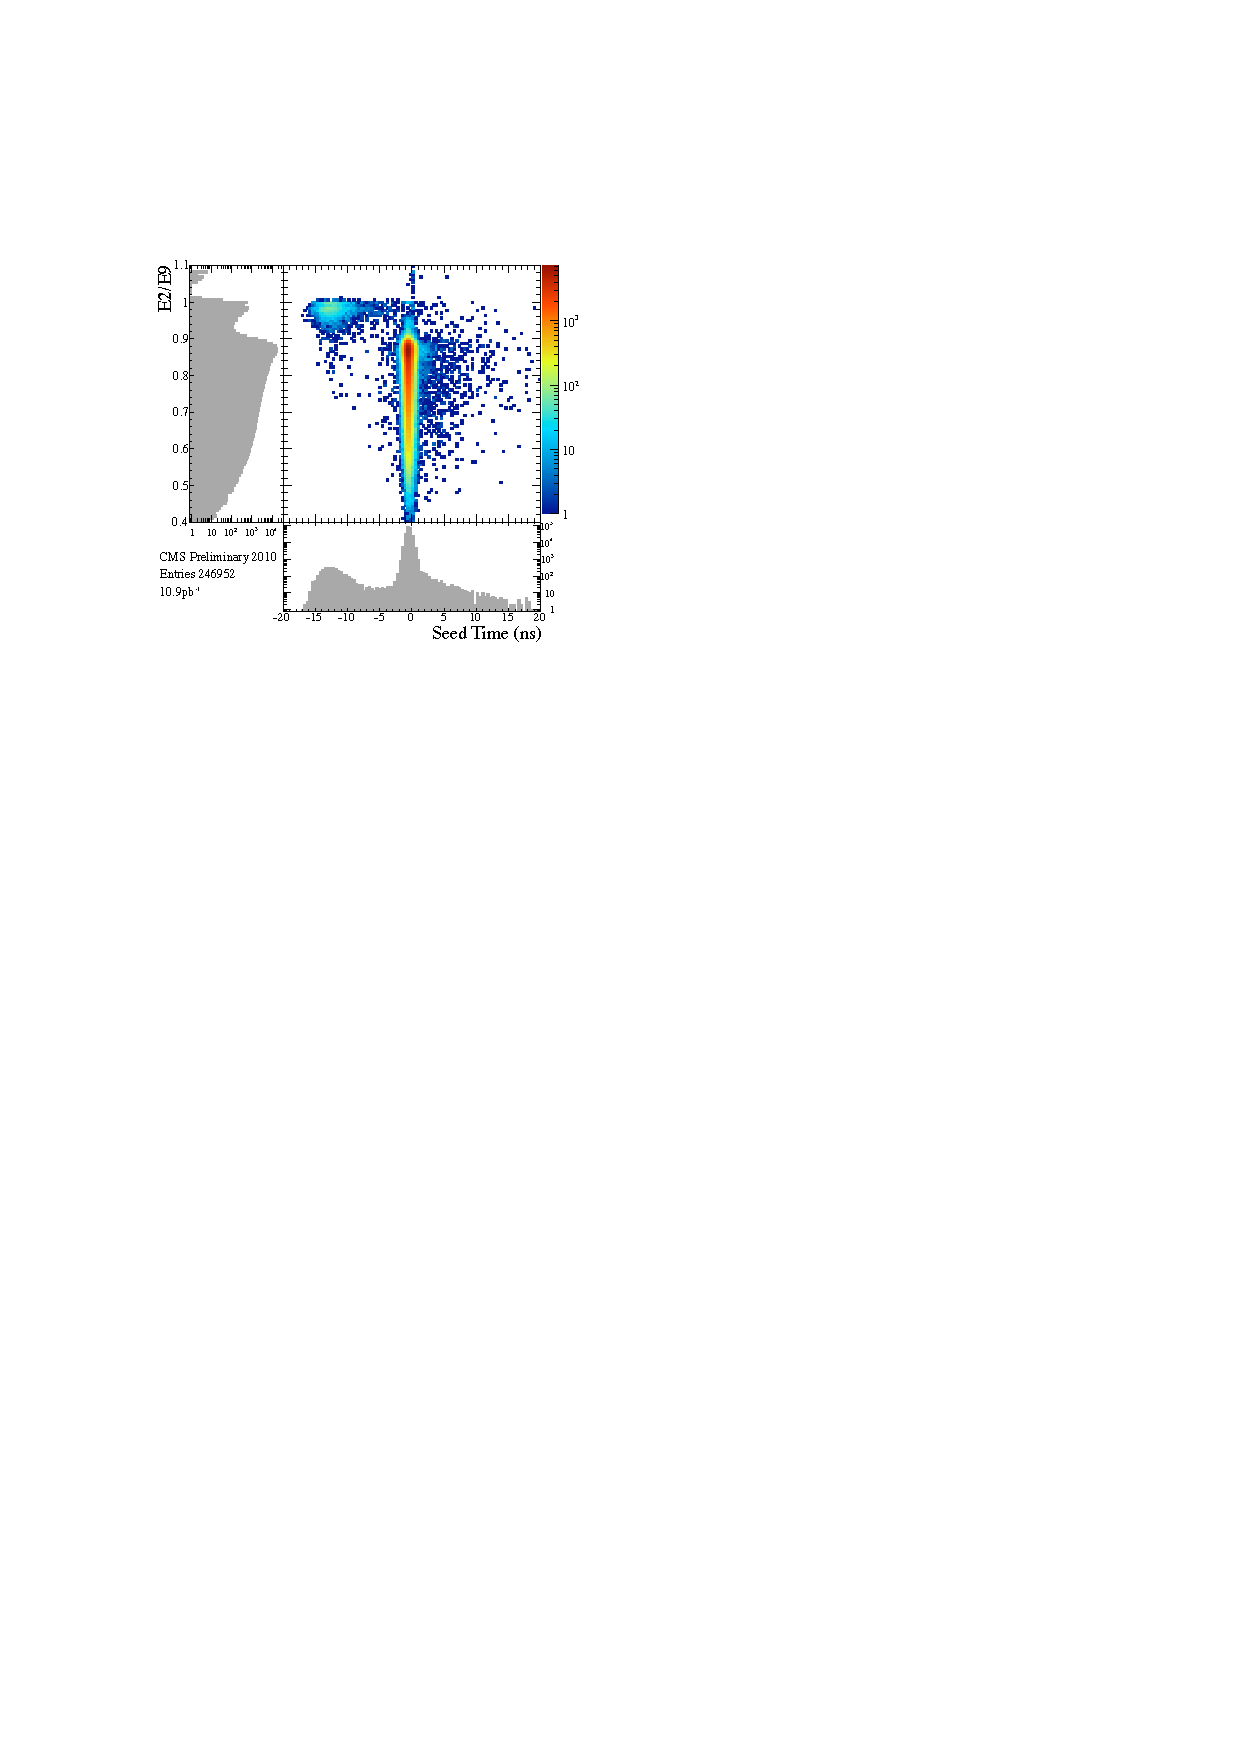
\includegraphics[width=\textwidth]{spikes.pdf}
\end{center}
\caption{A plot of e2/e9 vs seed time to show how double crystal ECAL spikes are
vetoed.}
\label{fig:spikes}
\end{figure}

$\HT$, the scalar sum of the transverse momentum of all the objects in the 
event, is used as a measure of the energy scale of the event. There is a $\HT$ 
cut because strongly produced SUSY events have high $\HT$. The value of this cut
is motivated by the desire for the trigger to be fully efficiency for the event
selection. Figure \ref{fig:Trigger_Efficiency} shows that the trigger becomes
fully efficient in HT at around $400\unit{GeV}$. \\

The $\geq 2$ jets cut is well motivated from the SUSY perspective: strongly
produced SUSY events start with two squarks/gluinos each of which decay to a 
quark/gluon (which forms a jet in the detector) and the next SUSY particle in 
the mass hierarchy. Parameter points with high gluino mass tend to have only 2 
jets while those with high squark mass tend to have at least 4 jets. \\

In strongly produced Gauge Mediated SUSY Breaking the Next-to-Lightest SUSY 
Particle (NLSP) is the neutralino ($\tilde{\chi}^{0}$) which decays to a photon 
and a gravitino. At least two photons are expected in each SUSY event. However, 
due to the high activity in these events, photons often fall inside the cone of
a jet and so only one photon is reconstructed. Hence the $\geq 1$ photon cut. \\

The search is done in bins of $\MET$ and $\HT$, but an initial $\MET$ cut is
made to avoid the low $\MET$ bins where there is no sensitivity due to the huge
amount of background. Figure \ref{fig:met_threshold} shows the signal efficiency
and the background rejection as a function of $\MET$ cut.

\begin{figure}
\begin{center}
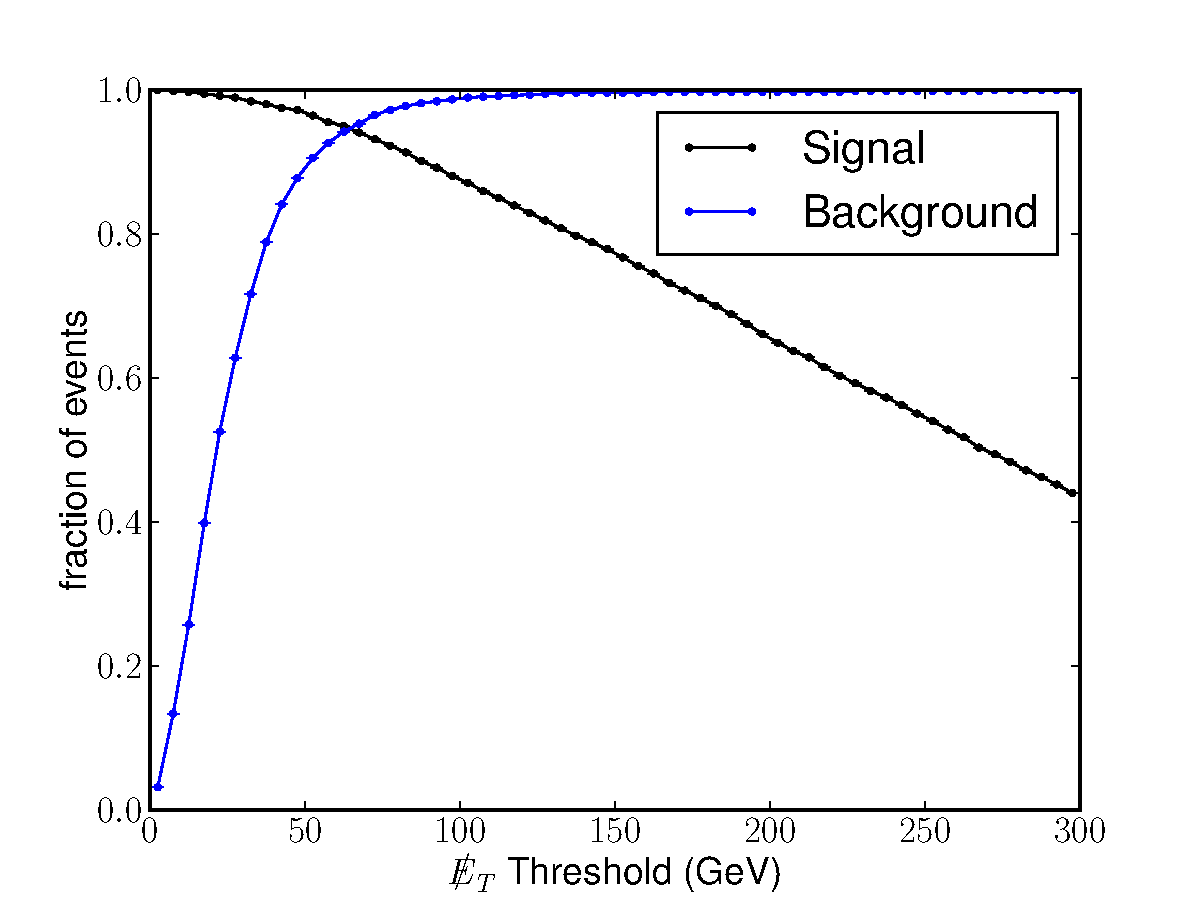
\includegraphics[width=0.7\textwidth]{MET_Threshold.pdf}
\end{center}
\caption{The signal efficiency (black) and background rejection (blue) as a
function of $\MET$ cut.}
\label{fig:met_threshold}
\end{figure}
